% ============================================================
%  KCMamba: Kalman-vezérelt állapottér-modell idősor-előrejelzésre
%  ELTE Informatikai Kar – TDK-dolgozat (37. OTDK)
%  Sablon: mcserep/elteikthesis v2.4  (MIT Licence)
%  Letöltés: bash setup.sh
% ============================================================
\documentclass[
    % parspace,   % bekezdések közötti extra közök
    % noindent,   % nincs behúzás
    % nohyp,      % nincs szóelválasztás
    % twoside,    % kétoldalas nyomtatás
    % draft,      % vázlat (gyors fordítás, képek nélkül)
    % final,      % végleges (TODO-k elrejtve)
]{elteikthesis}[2024/04/26]

% Dokumentum metaadatok
\title{KCMamba: Kalman-vezérelt szelektív\\
       állapottér-modell robusztus\\
       idősor-előrejelzésre}
\date{2026. május}

\author{Kovács András}
\degree{programtervező informatikus BSc, III. évfolyam}

\supervisor{Kristian Fenech Arian}
\affiliation{oktató}
% \extsupervisor{Külső Témavezető}
% \extaffiliation{...}

\university{Eötvös Loránd Tudományegyetem}
\faculty{Informatikai Kar}
\department{Mesterséges Intelligencia Tanszék}
\city{Budapest}
\logo{elte_cimer_szines}   % images/elte_cimer_szines.pdf

% Cellaszínezéshez (04_kiserletek.tex táblázatokban)
\PassOptionsToPackage{table}{xcolor}
\usepackage{colortbl}



% Hosszú kód-/parancssorok automatikus tördelése
\usepackage{fvextra}
\DefineVerbatimEnvironment{verbatim}{Verbatim}{breaklines=true,breakanywhere=true,fontsize=\footnotesize}

% Hosszú \texttt{...} útvonalak/azonosítók ne lógjanak ki a margón
\setlength{\emergencystretch}{3em}

% Use case diagramhoz
\usepackage{tikz}
\usetikzlibrary{shapes.geometric, positioning, fit, calc}

% Irodalomjegyzék forrása
\addbibresource{bib/references.bib}

% ============================================================
\begin{document}
% ============================================================

\documentlang{hungarian}

% Teendők listája (csak draft módban hasznos), véglegesben töröljük
%\listoftodos[\todolabel]

% ─── KÜLSŐ BORÍTÓ (OTDK előírás: „TDK-dolgozat" felirat + szerző neve) ───────
\begin{titlepage}
    \vspace*{\fill}
    \begin{center}
        {\Huge\bfseries TDK-dolgozat}\\[2.5cm]
        {\LARGE KCMamba: Kalman-vezérelt szelektív\\[0.4em]
                állapottér-modell robusztus\\[0.4em]
                idősor-előrejelzésre}\\[3cm]
        {\Large Kovács András}\\[0.5cm]
        {\large programtervező informatikus BSc, III. évfolyam}\\[2cm]
        {\large Eötvös Loránd Tudományegyetem\\[0.3em]
                Informatikai Kar}\\[0.8cm]
        {\large Budapest, 2026. május}
    \end{center}
    \vspace*{\fill}
\end{titlepage}

% Belső címlap (kötelező: intézmény, kar, tanszék, szerző, évfolyam, témavezető)
\maketitle

% Kivonat (kötelező)
\chapter*{Kivonat}
\addcontentsline{toc}{chapter}{Kivonat}

Ez a szakdolgozat a \textbf{KCMamba} (Kalman Core-Attention Mamba)
architektúrát mutatja be, amely differenciálható Kalman-szűrési mechanizmust
integrál a Mamba szelektív állapottér-modellbe (SSM) a zajrobusztus
idősor-előrejelzés érdekében. A javasolt architektúra tanult $Q_\text{net}$-,
$R_\text{net}$- és $K_\text{net}$-alhálózatokat alkalmaz, amelyek adaptívan
szabályozzák a mérési és folyamatzaj arányát, ezáltal a modell zajmentes
adatokon passzív előrejelzőként, zajosított bemeneten aktív szűrőként viselkedik.

Empirikus értékelést végzünk három nyilvános LTSF-adatkészleten
(Exchange-Rate, ETTh1, ETTh2), szintetikusan zajosított
($\sigma \in \{0, 1, 3, 5\}$) és alacsony adatbőségű (stride $\in \{1, 16\}$)
körülmények között.

Az Exchange-Rate adatkészleten végzett 3-mag kísérletben ($s=16$)
a KCMamba átlagos MSE-degradációja $\sigma{=}0$-tól $\sigma{=}5$-ig
$+1\,528\%$, a Fair Mambáé $+28\,234\%$, ami $18{,}5\times$-os stabilitási
különbséget jelent; a legsúlyosabb konfigurációban ($s{=}16$, $\sigma{=}5$)
a KCMamba MSE-je $1{,}41$, a Fair Mambáé $22{,}72$.
Az ablációs vizsgálat kimutatta, hogy a tanult $K$-gain elhagyása
a degradációt $2{,}4\times$-ra növeli, ezzel azonosítva a
$Q_\text{net}/R_\text{net}$ alhálózatokat mint a robusztusság
elsődleges forrását.

A szakdolgozat a teljes szoftverrendszer leírását is tartalmazza: egy aszinkron,
eseményvezérelt kereskedési motort hexagonális architektúrában, visszatesztelő
keretrendszert és élő Binance-kereskedési adaptert.

\cleardoublepage

% Abstract (angol kivonat, kötelező)
\chapter*{Abstract}
\addcontentsline{toc}{chapter}{Abstract}

This thesis presents \textbf{KCMamba} (Kalman Core-Attention Mamba),
a hybrid neural architecture that integrates a differentiable Kalman filtering
mechanism into the Mamba selective state-space model (SSM) for noise-robust
time series forecasting. The proposed architecture employs learned
$Q_\text{net}$, $R_\text{net}$, and $K_\text{net}$ subnetworks that adaptively
regulate the ratio of process and measurement noise, enabling the model to
behave as a passive predictor on clean data and as an active filter under noisy
conditions.

We conduct empirical evaluation on three public LTSF benchmarks
(Exchange-Rate, ETTh1, ETTh2) under synthetically injected noise
($\sigma \in \{0, 1, 3, 5\}$) and low data-availability regimes
(stride $\in \{1, 16\}$).

In the Exchange-Rate benchmark ($s=16$, 3-seed experiment), KCMamba's average
MSE degradation from $\sigma{=}0$ to $\sigma{=}5$ is $+1\,528\%$, compared
to $+28\,234\%$ for Fair Mamba, an $18.5\times$ stability gap; in the
hardest configuration ($s{=}16$, $\sigma{=}5$) KCMamba achieves MSE $1.41$
versus $22.72$ for Fair Mamba. The ablation study identifies the
$Q_\text{net}/R_\text{net}$ subnetworks as the primary source of robustness:
removing the learned $K$-gain increases degradation by $2.4\times$.

The thesis also describes the complete production software system: an
asynchronous, event-driven trading engine built in a hexagonal architecture,
a backtesting framework, and a live Binance trading adapter.

\cleardoublepage

% Tartalomjegyzék (kötelező)
\tableofcontents
\cleardoublepage

% ============================================================
%  FŐSZÖVEG
% ============================================================

% ============================================================
%  1. fejezet, Bevezetés
% ============================================================
\chapter{Bevezetés}
\label{ch:intro}

Az idősor-előrejelzés a gépi tanulás egyik kiterjedten kutatott
részterülete, amelynek gyakorlati jelentőségét a valós adatok szinte
kivétel nélkül jelen lévő zajossága adja. Szenzorkiesések, aggregációs
torzítások és piaci mikrostruktúra-zaj egyaránt rontják a jel/zaj arányt,
amelyre a kurrens modellek érzékenynek bizonyulnak.
A hosszú távú idősor-előrejelzés (LTSF) feladata ennél is nehezebb:
adott $L$ hosszúságú előzmény alapján kell becsülni a következő $H$ lépést,
ahol $H$ nagyságrendileg elérheti vagy meghaladhatja $L$-et.

\section{Motiváció}

A modern szekvencia-model-családok, a Mamba-alapú szelektív állapottér-modellek
~\cite{gu2021s4,gu2023mamba} és a klasszikus rekurrens hálózatok~\cite{hochreiter1997lstm}
az adatminőségi problémát implicit általánosítás révén kezelik: a zaj- és
jelkomponens szétválasztását kizárólag az adatvezérelt reprezentációtanulásra
bízzák.
Zajmentes adatokon ez az eljárás kielégítően teljesít, ám a megnövelt
zajszintre való általánosítóképesség empirikusan nem garantált.

A Kalman-szűrő~\cite{kalman1960new} ezzel szemben \emph{explicit}
statisztikai modellt állít fel a folyamatzajra ($Q$) és a mérési zajra ($R$),
és ezek arányából származtat egy $K$ gain együtthatót, amely az
előzmény-állapot és az aktuális megfigyelés közötti optimális súlyozást
határozza meg. Ennek az induktív torzításnak egy differenciálható
neurális hálózatba történő beépítése elméleti szempontból ígéretes
megközelítés a zajrobusztusság növelésére.

Ezen megfontolásra épül a jelen szakdolgozatban bemutatott \textbf{KCMamba}
architektúra.

\section{Célkitűzések}

Három konkrét kérdést vizsgálunk:

\begin{enumerate}
    \item Versenyképes-e a KCMamba tiszta adatokon a standard LTSF
          modellekkel szemben?
    \item Mekkora MSE-degradációt szenvednek el a modellek szintetikusan
          zajosított adatokon ($\sigma \in \{0, 1, 3, 5\}$)?
    \item Kevés tréning-ablak (stride $\in \{1, 16\}$) esetén melyik
          architektúra generalizál jobban?
\end{enumerate}

\section{Hozzájárulások}

\begin{itemize}
    \item A \textbf{KCMamba} architektúra leírása: tanult $Q_\text{net}$,
          $R_\text{net}$, $K_\text{net}$ alhálózatok differenciálható
          Kalman-szűrőn belül, párhuzamos prefix-scan GPU-implementációval.
    \item Mérések arról, hogy a tanult $K$ valóban adaptívan változik a
          zajszinttel: $\sigma=0$-nál $K \approx 0{,}71$ (passzív átengedés),
          $\sigma=5$-nél $K \approx 0{,}07$ (erős szűrés).
    \item Összehasonlítás három adatkészleten (Exchange-Rate, ETTh1, ETTh2):
          a Fair Mamba átlag $+28\,234\%$ MSE-degradációt mutat zajjal,
          a KCMamba $+1\,528\%$-ot.
    \item Nyílt forráskódú implementáció (Python/PyTorch/CUDA) és egy
          aszinkron kereskedési rendszer a modell deployálásához.
\end{itemize}

\section{Dolgozat felépítése}

A~\ref{ch:irodalom}. fejezet összefoglalja a Kalman-szűrő, az SSM-ek és
az LTSF-kutatás releváns irodalmát.
A~\ref{ch:architektura}. fejezet ismerteti a KCMamba architektúrát
és matematikai hátterét.
A~\ref{ch:kiserletek}. fejezetben a kísérleti beállítás és az eredmények
szerepelnek.
A~\ref{ch:implementacio}. fejezet a megvalósított szoftverrendszert
tárgyalja.
Az~\ref{ch:osszegzes}. fejezet levonja a következtetéseket.

\cleardoublepage

% ============================================================
%  2. fejezet, Irodalmi háttér
% ============================================================
\chapter{Irodalmi háttér}
\label{ch:irodalom}

\section{Kalman-szűrő és általánosításai}
\label{sec:kalman}

A Kalman-szűrő~\cite{kalman1960new} minimális varianciájú, torzítatlan,
lineáris becslő olyan rendszerekre, amelyek $x_t \in \mathbb{R}^n$ állapota
Gauss-zajjal perturbált lineáris dinamikai modell szerint fejlődik:
\begin{align}
    x_t &= F x_{t-1} + w_t, & w_t &\sim \mathcal{N}(0, Q), \label{eq:kf_process}\\
    y_t &= H x_t   + v_t,   & v_t &\sim \mathcal{N}(0, R), \label{eq:kf_measure}
\end{align}
ahol $F$ az állapotátmeneti mátrix, $H$ a mérési mátrix,
$Q \in \mathbb{R}^{n \times n}$ a folyamatzaj-kovariancia, és
$R \in \mathbb{R}^{m \times m}$ a mérési-zaj-kovariancia.
A szűrő két felváltva ismétlődő fázisban működik.

Az \emph{előrejelzési lépésben} (időfrissítés), mielőtt a $y_t$ mérés
megérkezne, a szűrő az állapotbecslést és a hibakovariancát előrevetíti:
\begin{align}
    \hat{x}_{t|t-1} &= F \hat{x}_{t-1|t-1}, \label{eq:kf_predict_x}\\
    P_{t|t-1}       &= F P_{t-1|t-1} F^\top + Q, \label{eq:kf_predict_P}
\end{align}
ahol $P_{t|t-1} \in \mathbb{R}^{n \times n}$ az előrejelzett hibakováriancia.
Nagy $P_{t|t-1}$ értéke magas előrejelzési bizonytalanságot jelez. Nagy $Q$ azt jelenti,
hogy az állapot gyorsan és kiszámíthatatlanul változik.

A \emph{korrekciós lépésben} (mérésfrissítés), amint a $y_t$ megfigyelés
megérkezik, a szűrő az \emph{innováció} $e_t = y_t - H\hat{x}_{t|t-1}$
alapján korrigálja becslését, a Kalman-gain $K_t$ által súlyozva:
\begin{align}
    K_t           &= P_{t|t-1} H^\top \bigl(H P_{t|t-1} H^\top + R\bigr)^{-1},
                     \label{eq:kalman_gain}\\
    \hat{x}_{t|t} &= \hat{x}_{t|t-1} + K_t e_t, \label{eq:kalman_update}\\
    P_{t|t}       &= (I - K_t H)\,P_{t|t-1}. \label{eq:kf_update_P}
\end{align}
A~\eqref{eq:kalman_gain}. egyenlet a zaj--jel-egyensúly alapvető összefüggését tükrözi.
Ha az $R$ mérési zaj nagy az előrejelzett $H P_{t|t-1} H^\top$
kovarianciához képest, a nevező dominál és $K_t \to 0$: a szűrő nem bízik
a mérésben, és az előzmény-állapotra támaszkodik. Ha $R \to 0$, akkor
$K_t \to H^{-1}$, és a megfigyelés majdnem teljesen felülírja az állapotot.

A skaláris esetben ($F = H = 1$) a gain egyszerűsödik:
\begin{equation}
    K_t = \frac{P_{t|t-1}}{P_{t|t-1} + R}.
    \label{eq:kalman_gain_scalar}
\end{equation}
Stacionárius feltételek mellett a $P_{t|t-1}$ hibakováriancia egy fix
$\bar{P}$ értékre konvergál, és az egyensúlyi gain kizárólag a $Q/R$
aránytól függ: magas folyamatzaj ($Q$) a $K$-t $1$ felé tolja (bízzunk
a mérésben), alacsony $Q/R$ arány $K$-t $0$ felé tolja (bízzunk
a modellben). (\ref{sec:kalman_gain}. szakasz).

\subsection{Tanult Kalman-szűrők}

A neurális Kalman-irodalomban a $F, H, Q, R$ mátrixokat neurális hálózatokkal
paraméterezik~\cite{krishnan2015deep,fraccaro2017disentangled}.
A \emph{Deep Kalman Filter}~\cite{krishnan2015deep} nemlineáris átmenetet
enged meg, a \emph{Kalman Variational Autoencoder}~\cite{fraccaro2017disentangled}
a latens állapotok szétválasztott reprezentációját tanítja.
A KCMamba ezeken az elveken épít, de nem autoencoderként, hanem
szekvencia-előrejelzőként.

\section{Állapottér-modellek}
\label{sec:ssm}

\subsection{S4}

Az S4 (Structured State Spaces for Sequences)~\cite{gu2021s4} egy
folytonos-idejű állapottér-modellből indul ki, amelyben egy $d$-dimenziós
bemeneti sorozatot egy $N$-dimenziós látens dinamikán keresztül modellez:
\begin{align}
    h'(t) &= A h(t) + B u(t), \\
    y(t) &= C h(t),
\end{align}
ahol $A \in \mathbb{R}^{N \times N}$ az állapotátmeneti mátrix, $B \in \mathbb{R}^{N \times d}$
a bemeneti projekció, $C \in \mathbb{R}^{d \times N}$ a kimeneti projekció,
és $h(t) \in \mathbb{R}^N$ a látens állapot.
Diszkretizálva egy $\Delta$ időlépéssel:
\begin{equation}
    h_t = \bar{A}\, h_{t-1} + \bar{B}\, u_t, \quad y_t = C\, h_t,
\end{equation}
ahol $\bar{A} = e^{\Delta A}$ és $\bar{B} \approx (\Delta A)^{-1}(e^{\Delta A} - I) \Delta B$.
Az S4 kulcsinnovációja az $A$ mátrix HiPPO-inicializációja, amely
az állapotnak polinomiális bázisú hosszú távú memóriát biztosít.
A konvolúciós nézet, $\bar{K} = (C\bar{B}, C\bar{A}\bar{B}, \ldots, C\bar{A}^{T-1}\bar{B})$
kernel, lehetővé teszi, hogy a tanítás $O(T \log T)$-ben
gyors Fourier-transzformációval (FFT) végezhető, míg az inferencia a rekurrens formában $O(1)$ memóriával
fut lépésenként.

\subsection{Mamba}

A Mamba~\cite{gu2023mamba} az S4 alapjaira építve bevezeti az
\emph{input-függő szelektivitást}: míg az S4-ben az $A$, $B$, $C$
mátrixok rögzítettek a teljes szekvenciára, a Mamba ezeket az aktuális
bemenettől függővé teszi. Ez a szelektivitás a lényege: a modell
minden időlépésben eldönti, mit őrizzen meg az állapotban és mit
felejtsen el. A bemeneti projekciós mátrix
$B(u_t) \in \mathbb{R}^{N \times d}$, a kimeneti projekció
$C(u_t) \in \mathbb{R}^{d \times N}$ és az időléptékező
$\Delta(u_t) \in \mathbb{R}^d$ mindegyike az aktuális
$u_t \in \mathbb{R}^d$ bemeneti vektortól függ:
\begin{equation}
    h_t = \overline{A}(u_t)\, h_{t-1} + \overline{B}(u_t)\, u_t,
    \quad y_t = C(u_t)\, h_t,
    \label{eq:mamba_recurrence}
\end{equation}
ahol $h_t \in \mathbb{R}^N$ a látens állapotvektor ($N$ az állapotméret),
$\overline{A}(u_t) = e^{\Delta(u_t) A}$ és
$\overline{B}(u_t) \approx \Delta(u_t) B$ a $\Delta$ alapján diszkretizált
mátrixok.
A modell így szelektíven dönti el, hogy a bemeneti sorozat melyik részét
tárolja tartósan az állapotban, és melyiket hagyja figyelmen kívül.
Hardver-barát párhuzamos prefix-scan implementációval $O(T)$ memória- és
időkomplexitást ér el.

\subsection{Fair Mamba}

Az összehasonlítási alap, amelyet \emph{Fair Mamba} névvel illetünk,
egy csatornánkénti (\emph{channel-wise}) Mamba, amelyet a KCMamba-éval
azonos hiperparaméterekkel és tanítási protokoll szerint tanítunk.
A \emph{fair} jelző arra utal, hogy a paraméterbudget és az adatmennyiség
azonos, így az eredménybeli különbség kizárólag az architektúrából fakad.

\section{Hosszú távú idősor-előrejelzés}
\label{sec:ltsf}

\subsection{Problémaformulázás}

A hosszú távú idősor-előrejelzés (LTSF) egy
$\mathbf{X} = (x_1, \ldots, x_L) \in \mathbb{R}^{L \times d}$
bemeneti ablakot tekint, amelynek $L$ historikus lépése $d$ csatornán van megadva,
és $\hat{\mathbf{X}} = (\hat{x}_{L+1}, \ldots, \hat{x}_{L+H}) \in \mathbb{R}^{H \times d}$
előrejelzését kívánja adni a következő $H$ lépésre.
A cél a normált átlagos négyzetes hiba minimalizálása:
\begin{equation}
    \mathrm{MSE} = \frac{1}{H d}
        \sum_{h=1}^{H} \sum_{j=1}^{d}
        \frac{(x_{L+h,j} - \hat{x}_{L+h,j})^2}{\mathrm{Var}(x_{\cdot,j})},
    \label{eq:mse}
\end{equation}
ahol a csatornánkénti varianciával való normálás különböző skálájú
adatkészletek eredményeit összehasonlíthatóvá teszi.
A \emph{hosszú távú} jelző a $H \geq L$, illetve $H$ és $L$ hasonló nagyságrendű esetét jelöli:
az ilyen feladatban a modellnek a visszatekintési ablakán jócskán túlra kell előrejelezni,
ez pedig lényegesen nehezebb, mint a rövid távú eset, ahol $H \ll L$.

\subsection{Referenciamodellek}

\emph{Informer}~\cite{zhou2021informer} volt az első, kifejezetten hosszú
távú előrejelzésre tervezett Transformer-változat. A standard önfigyelés
$O(L^2)$ idő- és memóriakomplexitása hosszú bemeneti ablakoknál
elfogadhatatlanul magas. Az Informer ezt \emph{ProbSparse attention}\textrm{-}tel
orvosolja: KL-divergencia-becslés alapján azonosítja az $O(\log L)$
leginformatívabb lekérdező pozíciót, ezzel $O(L \log L)$-re csökkenti
a komplexitást. Disztillációs művelet felezi a szekvenciahosszat az
enkoderblokkok között, így több ezer lépéses visszatekintési ablakok is
kezelhetők.

\emph{Autoformer}~\cite{wu2021autoformer} minden sorozatot egy
trendkomponensre (mozgóátlag-kernellel becsülve) és egy szezonális
maradéktagra bont, és a Transformert kizárólag a maradéktagokra alkalmazza.
Pontszorzat-figyelem helyett \emph{Auto-Korrelációs} mechanizmust
használ: megkeresi azt a $\tau$ késleltetést, amely maximalizálja
a lekérdező jel autokorrelációját, majd ezeken a késleltetési pozíciókon
összesíti az értékeket. A mechanizmus FFT-vel $O(L \log L)$ komplexitású,
és periodikus jelekre illeszkedő induktív torzítással rendelkezik.

\emph{DLinear}~\cite{zeng2023transformers} elveti az architekturális
bonyolultságot, és az előrejelzést minden visszatekintési ablakra
egyetlen lineáris réteggel állítja elő, opcionálisan trend-szezonális
felbontás után. Egyszerűsége ellenére a DLinear számos Transformer-változattal
azonos szinten teljesített, sőt azokat felülmúlta szabványos benchmarkokon,
bizonyítva, hogy az architekturális bonyolultság nem feltétele a jó
előrejelzési teljesítménynek. Referenciamodellként releváns marad, mert
minden új modellnek igazolnia kell, hogy a magasabb számítási ráfordítás
indokolt ehhez az egyszerű alapmodellhez képest.

\subsection{Adatkészletek}
\label{sec:datasets}

Az Exchange-Rate adatkészlet~\cite{lai2018modeling} nyolc valutaárfolyamot
tartalmaz, amelyeket 1990 és 2016 között napi szinten vettek fel,
csatornánként 7\,588 időlépéssel. Az árfolyam-adatok dinamikája majdnem egységgyök-jellegű: minden napi
változás véletlenszerű bolyongáshoz közelít, szinte elhanyagolható
vissza-átlagolással. Ez kemény feladatot jelent az autoregresszív modelleknek,
és természetes tesztkörnyezetet jelöl a Kalman-struktúra számára,
ahol a jel-zaj arány eleve alacsony.

Az ETTh1 és ETTh2 adatkészletek~\cite{zhou2021informer} kínai
transzformátorállomásokból gyűjtöttek óránkénti villamosenergia-terhelést
és olajhőmérsékletet két éven keresztül (17\,420 lépés, $d=7$ csatorna).
Az ETTh1 egyértelmű napi periodicitást mutat, az ETTh2 zajosabb és
szabálytalanabb. A két adatkészlet eltérő nehézségű tesztkörnyezetet
nyújt a zajrobusztusság kiértékeléséhez.

\section{Zajrobusztusság}
\label{sec:robustness}

Az idősor-modellek zajérzékenységének szisztematikus elemzése az
LTSF-irodalomban aláreprezentált terület.
A PatchTST~\cite{nie2022patchtst} patch-tokenizálással csökkenti a
szomszédos mintavételezési torzítást. Ennek közvetett zajcsökkentő hatása
van, bár nem ez az eljárás fő célkitűzése.

A jelen munkában az értékelési protokoll: $\tilde{x}_t = x_t + \varepsilon_t$,
ahol $x_t \in \mathbb{R}^d$ az eredeti idősorjel, $\varepsilon_t \sim \mathcal{N}(0, \sigma^2 I)$
additív Gauss-zaj ($\sigma > 0$ a szórás, $I \in \mathbb{R}^{d \times d}$
az egységmátrix), és $\sigma \in \{0, 1, 3, 5\}$ a vizsgált zajszintek halmaza.
A tanító- és teszthalmazt egyaránt azonos $\sigma$-val zajosítjuk,
tehát nem domain-shift-ről, hanem egyenletes adatminőség-romlásról van szó.

\cleardoublepage

% ============================================================
%  3. fejezet, KCMamba architektúra
% ============================================================
\chapter{A KCMamba architektúra}
\label{ch:architektura}

\section{Áttekintés}

A KCMamba (Kalman Core-Attention Mamba) egy hibrid neurális
architektúra, amely a Mamba SSM~\cite{gu2023mamba} rekurrens dinamikájába
egy differenciálható, tartalomfüggő Kalman-szűrő réteget integrál.
A modell nem rögzített $A$ felejtési faktorral dolgozik, hanem egy, a
bemenetből tanult $K$-gainből származtatott $A = 1-K$ együtthatót
használ az állapotfrissítésben. Ez lehetővé teszi, hogy az előzmény-
állapot és az aktuális megfigyelés közötti súlyozás a zajszintnek
megfelelően, adaptívan álljon be.

A modell két szintből épül fel: az alap feldolgozó egység a
\texttt{KCMambaBlock} (tartalom-függő Kalman-szűrés és állapotfrissítés),
fölötte a \texttt{KCMambaStack}: $N$ egymás utáni KC-blokk
cross-attention réteggel a végén.

\begin{figure}[H]
  \centering
  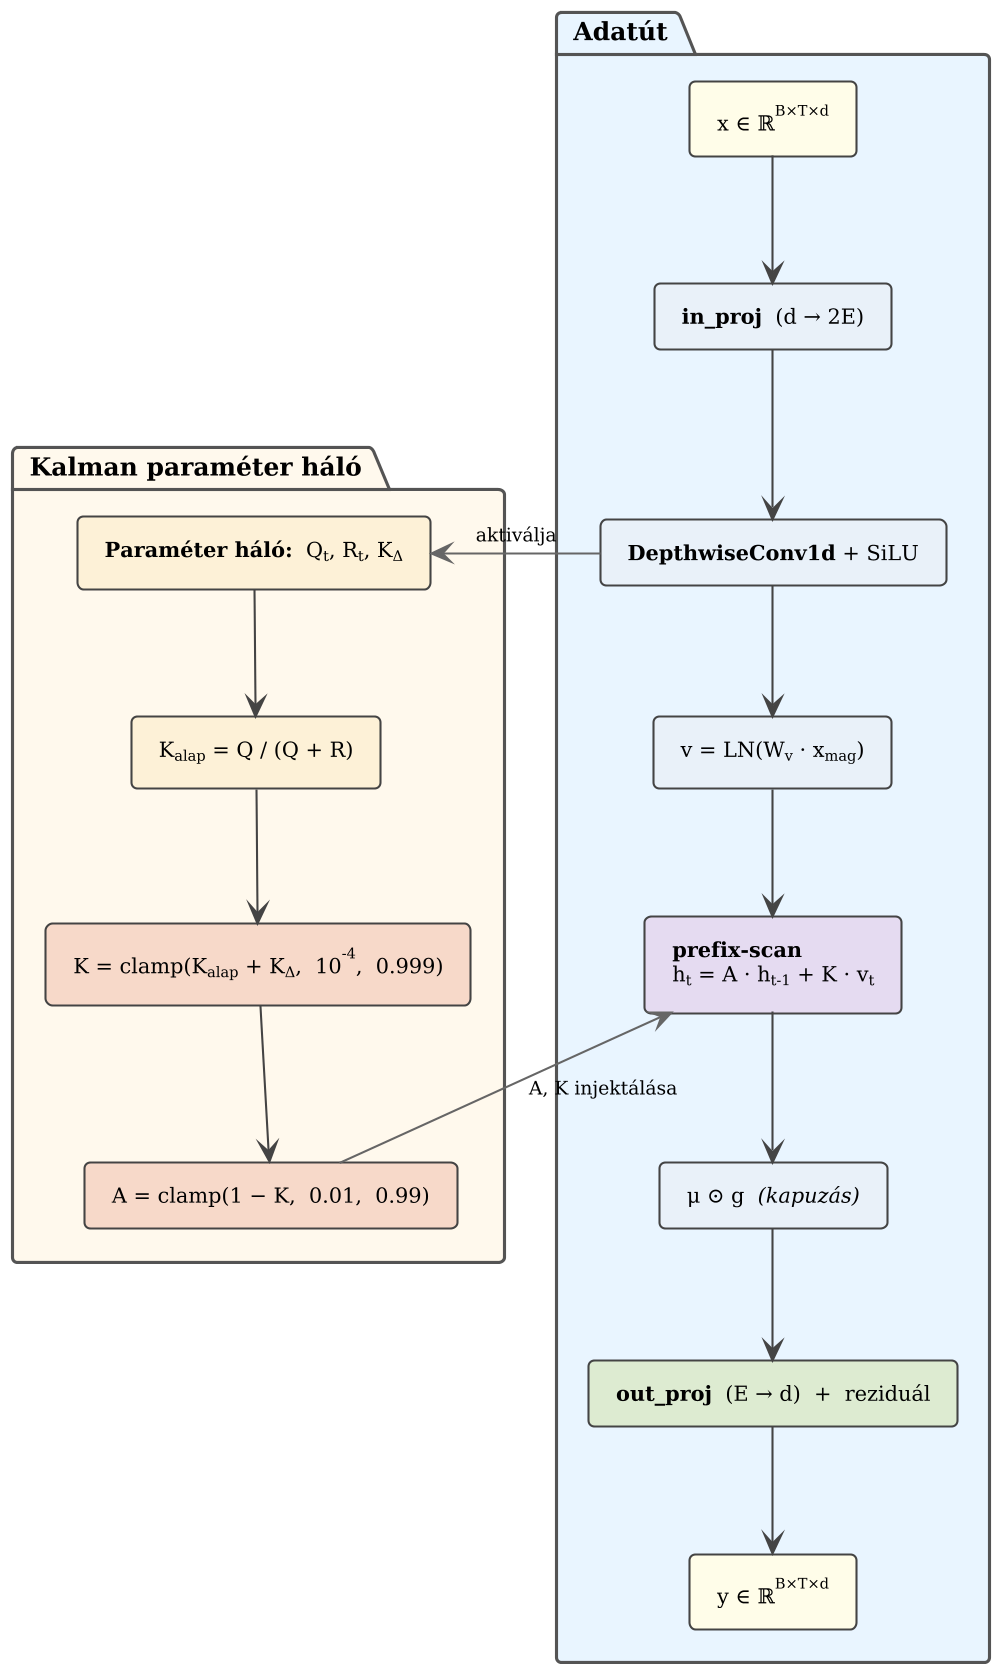
\includegraphics[width=\textwidth, height=0.85\textheight, keepaspectratio]{images/fig08_architecture_hu.png}
  \caption{A KCMamba blokk teljes adatfolyam-diagramja. A sárga blokkok
           ($Q_\text{net}$, $R_\text{net}$, $K_\text{net}$) tanítják a Kalman-statisztikákat,
           a lila blokkban történik a párhuzamos prefix-scan GPU-n $O(\log T)$
           szinkronizációval. A zöld blokkok a bemeneti és kimeneti projekciókat jelölik.}
  \label{fig:arch_overview}
\end{figure}

\section{KCMamba blokk}
\label{sec:kc_block}

Legyen a bemenő szekvencia $x \in \mathbb{R}^{B \times T \times d}$,
ahol $B$ a kötegméret, $T$ a szekvenciahossz, és $d$ a jellemzők száma.

\subsection{Bemeneti projekció és 1D-konvolúció}

A bemenetet két részre vetítjük egy lineáris réteggel,
majd SiLU aktivációs kapuzást alkalmazunk:
\begin{align}
    [x_\text{cw},\; x_\text{gate}] &= W_\text{in}\, x, \\
    \text{gate} &= \mathrm{SiLU}(x_\text{gate}),
\end{align}
ahol $W_\text{in} \in \mathbb{R}^{2d_\text{inner} \times d}$ a bemeneti projekciós
mátrix, $d_\text{inner}$ a belső csatornadimenzió, $x_\text{cw}$ a
Kalman-szűrési ághoz, $x_\text{gate}$ a kapuzáshoz továbbított csatorna,
és $\mathrm{SiLU}(z) = z \cdot \sigma(z)$ a Sigmoid Linear Unit aktiváció,
ahol $\sigma(z) = 1/(1+e^{-z})$ a logisztikus szigmoid.
A kétágú projekció két különböző szerepet tölt be.
Az $x_\text{cw}$ csatorna a Kalman-szűrési ág bemenete, míg az $x_\text{gate}$
csatorna a kimenet amplitúdójának független modulálásáért felel.
Ez a szétválasztás megakadályozza, hogy a kapuzási jel beavatkozzon a
Kalman-állapot dinamikájába.
A SiLU aktiváció ReLU-val szemben azért előnyös, mert sima és kis negatív
értékeket is megenged, ami a korai tanítás során javítja a gradiens-átmenetet.

A globális szekvenciális scan előtt az $x_\text{cw}$ csatornán egy depthwise
1D-konvolúció ($k=4$ kernel) biztosítja a lokális kontextus-integrációt:
\begin{equation}
    x_\text{core} = \mathrm{SiLU}\bigl(\mathrm{Conv1D}(x_\text{cw})\bigr).
\end{equation}
A konvolúció csatornánként egy szűrőt alkalmaz (depthwise), ezért mindössze
$k \cdot d_\text{inner}$ extra paramétert igényel, miközben
rövid-horizontú mintázatokat, például rövid-távú lendületet és trendirányokat,
ragad meg, mielőtt a Kalman-szűrő a teljes szekvenciát feldolgozza.

\subsection{Kalman-paraméter hálózatok}

Három kis, kétrétegű, teljesen összekötött alhálózat tanítja meg a Kalman-szűrő statisztikáit.
A $Q_\text{net}$ és $R_\text{net}$ hálózatok az időlépésenkénti
zajvarianciákat becslik:
\begin{align}
    Q_t &= \mathrm{softplus}(Q_\text{net}(x_\text{core})) \cdot
           \mathrm{softplus}(q_\text{scale}), \label{eq:Q_net}\\
    R_t &= \mathrm{softplus}(R_\text{net}(x_\text{core})) \cdot
           \mathrm{softplus}(r_\text{scale}). \label{eq:R_net}
\end{align}
ahol $Q_t > 0$ a \emph{folyamatzaj} becsült varianciája, vagyis az állapot-dinamikára
vonatkozó bizonytalanság, $R_t > 0$ a \emph{mérési zaj} becsült varianciája,
vagyis a bemeneti megfigyelés bizonytalansága,
$q_\text{scale},\, r_\text{scale} \in \mathbb{R}$ tanítható skalár
paraméterek, és $\mathrm{softplus}(z) = \ln(1+e^z) > 0$
garantálja a pozitivitást.
A $q_\text{scale} = -2{,}0$, $r_\text{scale} = 1{,}5$ inicializációk biztosítják,
hogy kezdetben $R \gg Q$, vagyis $K_\text{base} \approx 0.07$, ami erős szűrési
módot jelent alapértelmezésként.

Egy harmadik alhálózat, a $K_\text{net}$, szintén kétrétegű, teljesen összekötött Multi-Layer Perceptron,
és közvetlen reziduál-korrekciót nyújt a végső gainhez, ahogy azt a
\ref{sec:kalman_gain}.\ szakasz részletezi.
A $Q_\text{net}$/$R_\text{net}$ pár a lassan változó zajkörnyezetet modellezi,
míg a $K_\text{net}$ azonnali reakcióra képes gyors, tartalomfüggő eseményekre,
például hirtelen volatilitásnövekedésre vagy trendfordulóra, amelyekre
a zaj-arány becslése még nem alkalmazkodott.

\newpage
\subsection{Kalman-gain számítás}
\label{sec:kalman_gain}

Az alap Kalman-gain a folyamat- és mérési zaj \emph{arányából} következik,
ami a becsléselméleti steady-state Kalman-gain klasszikus képlete:
\begin{equation}
    K_{\text{base},t} = \frac{Q_t}{Q_t + R_t + \varepsilon},
    \label{eq:K_base}
\end{equation}
ahol $\varepsilon = 10^{-6}$ a nullával való osztást megelőző numerikus
stabilitási konstans.
Ha $Q \gg R$, azaz az állapot gyorsan változik, akkor $K \to 1$, és a modell szorosan
követi az aktuális megfigyelést. Ha $R \gg Q$, azaz a mérés zajos, akkor $K \to 0$,
és az előző állapot dominál.
Ez egy fizikailag értelmes, kontrollelméleti elvekre támaszkodó prior.

Ehhez járul egy tartalom-függő korrekció a $K_\text{net}$ alhálózattól,
ami olyan gyors rezsimváltások kezelésére képes, amelyekre a lassan
alkalmazkodó $Q/R$ arány még nem reagált:
\begin{equation}
    K_t = \mathrm{clamp}\Bigl(K_{\text{base},t} +
          0.3\bigl(\sigma_\text{sig}(K_\text{net}(x_\text{core})) - 0.5\bigr),\;
          [10^{-4},\; 0{,}999]\Bigr),
    \label{eq:K_final}
\end{equation}
ahol $\sigma_\text{sig}(\cdot) = 1/(1+e^{-(\cdot)})$ a logisztikus szigmoid
függvény, amelynek értékkészlete a $(0,1)$ nyílt intervallum, a $-0{,}5$ eltolás nullára centrálja
a korrekciót inicializáláskor, és a $0{,}3$ szorzó $(-0{,}15,\, +0{,}15)$-re
korlátozza a hatókörét.
A $[10^{-4},\, 0{,}999]$-re való vágás két degenerált esetet zár ki.
$K_t \approx 0$ befagyasztaná az állapotfrissítést, mivel nem integrálódna
új információ. $K_t \approx 1$ esetén a modell az előző lépés teljes memóriáját eldobná.

\subsection{Állapotfrissítés párhuzamos scan-nel}

Az $A_t = \mathrm{clamp}(1 - K_t, 0{,}01, 0{,}99)$ felejtési faktorral
a diszkrét Kalman-rekurzió:
\begin{align}
    h_t &= A_t \odot h_{t-1} + K_t \odot v_t, \label{eq:kc_recurrence}\\
    v_t &= \mathrm{LayerNorm}(W_v \, x_\text{core,t}), \nonumber
\end{align}
ahol $A_t \in (0,1)^{d_\text{inner}}$ a felejtési faktor vektora,
amelynél $A_t \to 1$ erős memóriát, $A_t \to 0$ erős frissítést jelent,
$\odot$ az elem-szintű (Hadamard) szorzás, $h_{t-1} \in \mathbb{R}^{d_\text{inner}}$
az előző lépés látens állapota, $v_t$ az aktuális értékvektor, és
$W_v \in \mathbb{R}^{d_\text{inner} \times d_\text{inner}}$ tanítható projekció.
A rekurzió hatékony kiértékelése a Blelloch-féle párhuzamos prefix-scan
algoritmussal~\cite{blelloch1990prefix} valósul meg:
\begin{align}
    A_\text{new}[t] &\leftarrow A[t] \cdot A[t-\text{step}], \\
    B_\text{new}[t] &\leftarrow B[t] + A_\text{orig}[t] \cdot B[t-\text{step}],
\end{align}
ahol $A[t]$ és $B[t]$ az asszociatív prefix-pár $(a_t, b_t)$ tagjai,
$a_t$ a halmozódó felejtési faktor, $b_t$ a halmozódó bemenet-összeg.
Ezek \emph{nem} azonosak az SSM $A$, $B$ mátrixaival,
és a lépésköz $\text{step} \in \{1, 2, 4, \ldots, T/2\}$ duplázódik.
A rekurzió $O(\log T)$ szinkronizációs lépéssel párhuzamosítható GPU-n.

\begin{figure}[H]
  \centering
  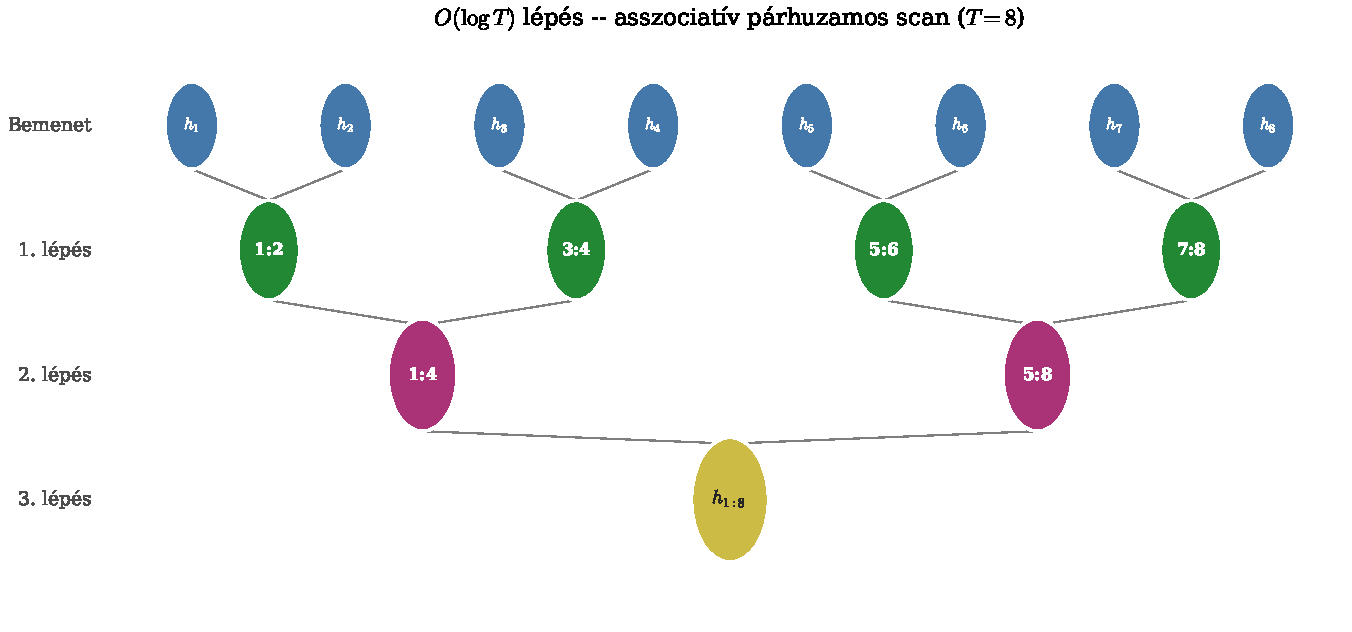
\includegraphics[width=\textwidth]{images/fig09_parallel_scan_hu.pdf}
  \caption{A Blelloch-féle párhuzamos prefix-scan vizualizációja 8 elemű
           szekvencián. Minden lépésben a $step$-nyi távolságú két elem
           kombinálódik.
           $\log_2 T = 3$ lépés után minden $h_t$ tartalmazza az előzmény-összesítést.
           Ez teszi lehetővé a szekvenciális állapotfrissítés hatékony GPU-s
           párhuzamosítását.}
  \label{fig:parallel_scan}
\end{figure}

\subsection{Összegzés és reziduál kapcsolat}

A Kalman-állapot-sorozat és a kapuzás kombinálja a kimenetet:
\begin{equation}
    y_\text{KC} = W_\text{out}(\mu \odot \text{gate}),
\end{equation}
ahol $\mu = (h_1, \ldots, h_T) \in \mathbb{R}^{T \times d_\text{inner}}$
az összes időlépés Kalman-állapota, $W_\text{out} \in \mathbb{R}^{d \times d_\text{inner}}$
a kimeneti projekció, és $\odot$ az elem-szintű szorzás.
Egy skalárkapuzással vezérelt reziduál kapcsolat biztosítja a gradiens
átmenő útját:
\begin{equation}
    \text{out} = y_\text{KC} + \sigma(b_\text{res}) \cdot
                 (W_\text{res}\,x - y_\text{KC}),
\end{equation}
ahol $b_\text{res} \in \mathbb{R}$ tanítható skalár, amelyet $-1{,}0$-ra
inicializálunk, így $\sigma(b_\text{res}) \approx 0{,}27$,
$W_\text{res}$ a reziduál projekció, és a kis $\sigma(b_\text{res})$
alaphelyzetben az SSM-ágat részesíti előnyben.

\section{KCMamba verem}
\label{sec:kc_stack}

A verem $N$ rétegből áll, pre-norm elrendezésű LayerNorm rétegekkel,
amelyek megakadályozzák az aktivációs skála sodródását.

A verem végére egy \emph{multi-scale cross-attention} réteget illesztünk.
Ennek oka, hogy a Mamba rekurrens dinamikája a rejtett állapotba a közelmúlt
lépéseit súlyozottan erősebben kódolja, mint a régmúlt szegmenseket.
Hosszú horizontú előrejelzésnél azonban a lassú trendekhez is hozzáférést
kell biztosítani.
A cross-attention lekérdezésként a jelenlegi állapotot összeveti a szekvencia
minden $s$-edik pozíciójából vett mintázatok (key/value) halmazával,
így rövid és hosszú időskálákat egyaránt számításba vesz:
\begin{equation}
    \text{out}[T] = h[T] + \mathrm{MHA}\bigl(h[T],\; h[{::s}],\; h[{::s}]\bigr),
\end{equation}
ahol $h[T] \in \mathbb{R}^{1 \times d}$ a legutolsó időlépés reprezentációja
és egyben a lekérdezés, $h[{::s}] \in \mathbb{R}^{\lfloor T/s \rfloor \times d}$
minden $s$-edik pozícióból vett alminta, amely a lassabb, durvább
időskálát képviseli kulcsként és értékként,
és $\mathrm{MHA}(\text{lekérdezés},\text{kulcs},\text{érték})$ a multi-head
cross-attention a megszokott értelemben~\cite{vaswani2017attention}.
\begin{figure}[H]
  \centering
  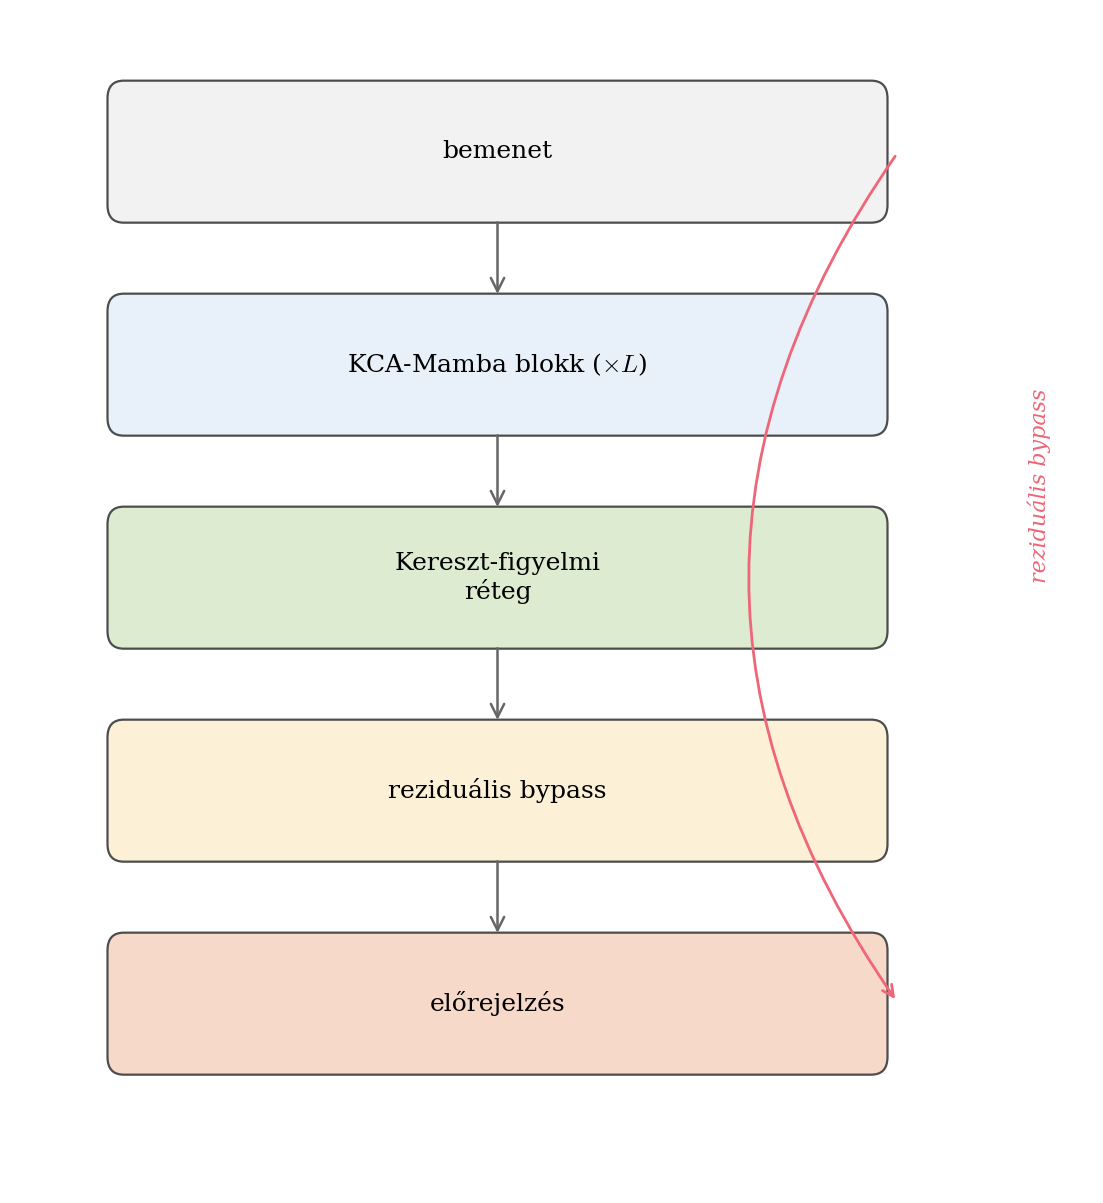
\includegraphics[width=0.55\textwidth, height=0.65\textheight, keepaspectratio]{images/kc_stack_diagram_hu.png}
  \caption{A KCMamba verem (stack) felépítése. A bemenettől a kimenetig az
           input projekció, 2 KC-blokk LayerNorm rétegekkel, output
           normalizáció, majd cross-attention réteg követi egymást a lassú ($s=4$)
           időskála integrálásához.}
  \label{fig:stack_diagram}
\end{figure}
\begin{figure}[H]
  \centering
  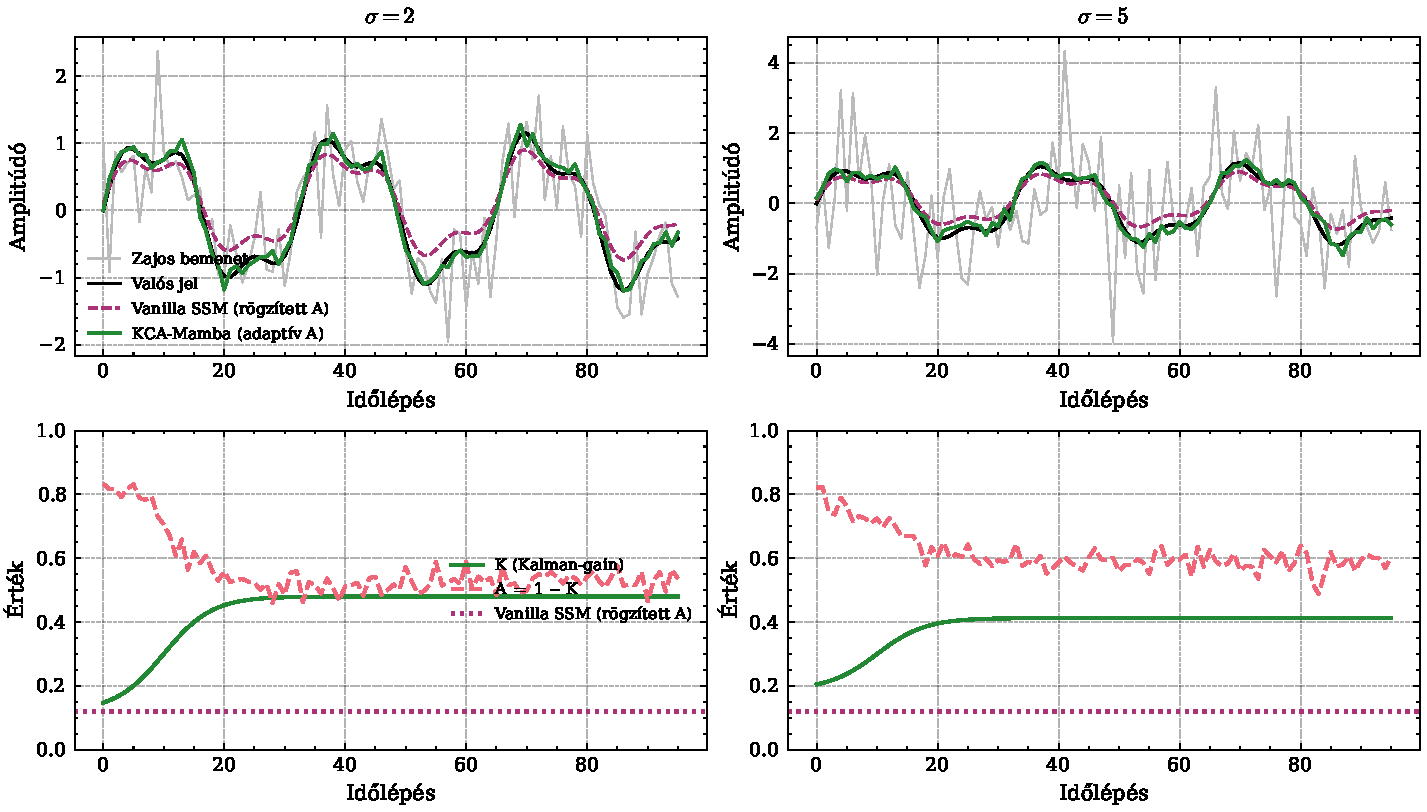
\includegraphics[width=\textwidth]{images/fig11_synth_mamba_hu.pdf}
  \caption{Szintetikus jel szűrése: \textbf{vanilla SSM} (standard Mamba, rögzített $A$)
           vs.\ \textbf{KCMamba} (adaptív $K$-gain) közepes ($\sigma=2$) és erős
           ($\sigma=5$) zajnál.
           \textit{Felső sorok:} az előrejelzett jel a valódihoz képest.
           A KCMamba szorosabban követ zajban is.
           \textit{Alsó sorok:} a tanult $K$-értékek időbeli változása.
           A vanilla SSM $A$-ja rögzített, a KCMamba $A$-ja adaptívan nő zajjal.}
  \label{fig:synth_mamba}
\end{figure}

\begin{figure}[H]
  \centering
  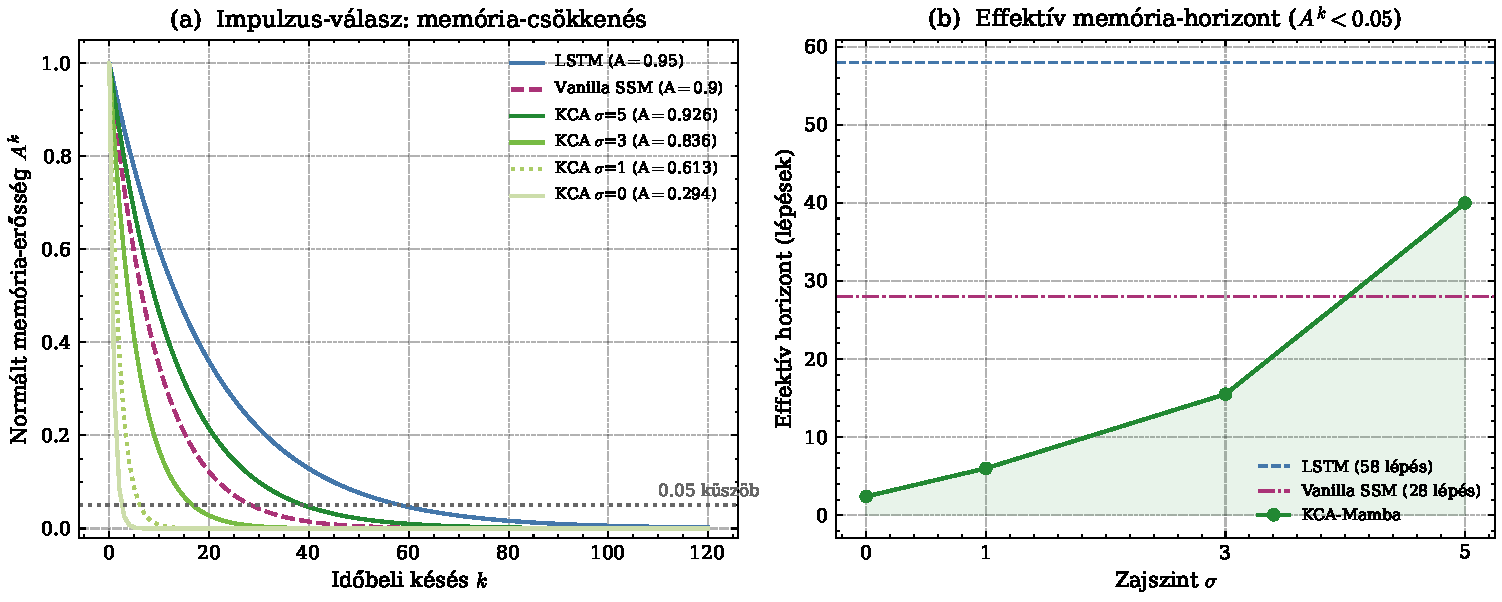
\includegraphics[width=\textwidth]{images/fig13_memory_retention_hu.pdf}
  \caption{\textbf{Bal:} Impulzus-válasz függvény: az állapot exponenciális csökkenése
           $h_k = A^k$ a $k$ késleltetés függvényében. A KCMamba $A$-értéke adaptívan
           nő a zajszinttel ($0.294 \to 0.926$), ezzel a memória-horizont
           is növekszik.
           \textbf{Jobb:} Effektív memória-horizont (az a lépésszám, ameddig
           $A^k > 5\%$) a zajszint függvényében. Az LSTM és vanilla SSM
           rögzített horizonttal rendelkeznek, a KCMamba zajban automatikusan
           hosszabb memóriát tart fenn.}
  \label{fig:memory_retention}
\end{figure}

\section{Paraméterkomplexitás}

\begin{table}[H]
    \centering
    \begin{tabular}{|l|r|r|r|}
        \hline
        \textbf{Modell} & \textbf{Paraméterek (k)} & \textbf{Rétegek} & \textbf{Állapotméret} \\
        \hline\hline
        LSTM            & 71{,}7 & 1 & 128 \\
        Fair Mamba      & 53{,}2 & 2 & H=4, D=32 \\
        KCMamba       & 46{,}1 & 2 & H=4, D=32 \\
        \hline
    \end{tabular}
    \caption{A kísérletekben használt modellek paraméterkomplexitása
             (medium méretkonfiguráció). A KCMamba kevesebb paraméterrel
             rendelkezik, mint a Fair Mamba, mivel a $Q_\text{net}/R_\text{net}/K_\text{net}$
             alhálózatok az SSM-blokkokból az erőforrásokat átirányítják.}
    \label{tab:params}
\end{table}

\newpage
\section{Összehasonlítás a standard Mamba-val}

A legfontosabb architekturális különbség a standard (vanilla) SSM és
a KCMamba között az $A$ felejtési faktor kezelésében keresendő.
A standard Mamba~\cite{gu2023mamba} az $A$ mátrixot a $\Delta$ időléptékű
paraméteren keresztül tanulja, de ez a reprezentáció nem különíti el a
jel- és zajkomponenst: $\Delta$ egyszerre jelöli ki az adatstruktúra
tanulási dinamikáját \emph{és} a zajszűrést.

A KCMamba ezt a kettősséget bontja meg egy explicit $Q/R$
zajtartomány-modell bevezetésével.
A $K = Q/(Q+R)$ arány határozza meg, hogy az állapotfrissítés az
aktuális mérésre vagy az előzmény-állapotra támaszkodik-e erősebben.
Magas zaj mellett ($\sigma=5$) $K \to 0.073$, azaz $A = 0.927$: a modell
erős memóriát tart fenn, és kiszűri a zajos méréseket
(erős szűrési mód).
Alacsony zaj mellett ($\sigma=0$) $K = 0.706$, és a modell az aktuális
megfigyelést követi (\emph{innovációs mód}).

Ezt a szintetikus teszten a \ref{fig:synth_mamba}.\ ábra demonstrálja.
A standard SSM rögzített $A=0.88$ értékkel dolgozik mindkét zajszinten,
míg a KCMamba $A$-ja a zajszinttel arányosan módosul (\ref{fig:memory_retention}.\ ábra).

\newpage
\section{Rendszerarchitektúra}
\label{sec:system_arch}

A KCMamba egy hexagonálisan strukturált kereskedési rendszerbe épül be.
A \ref{fig:system_arch}.\ ábra a főbb komponenseket mutatja:

\begin{figure}[H]
  \centering
  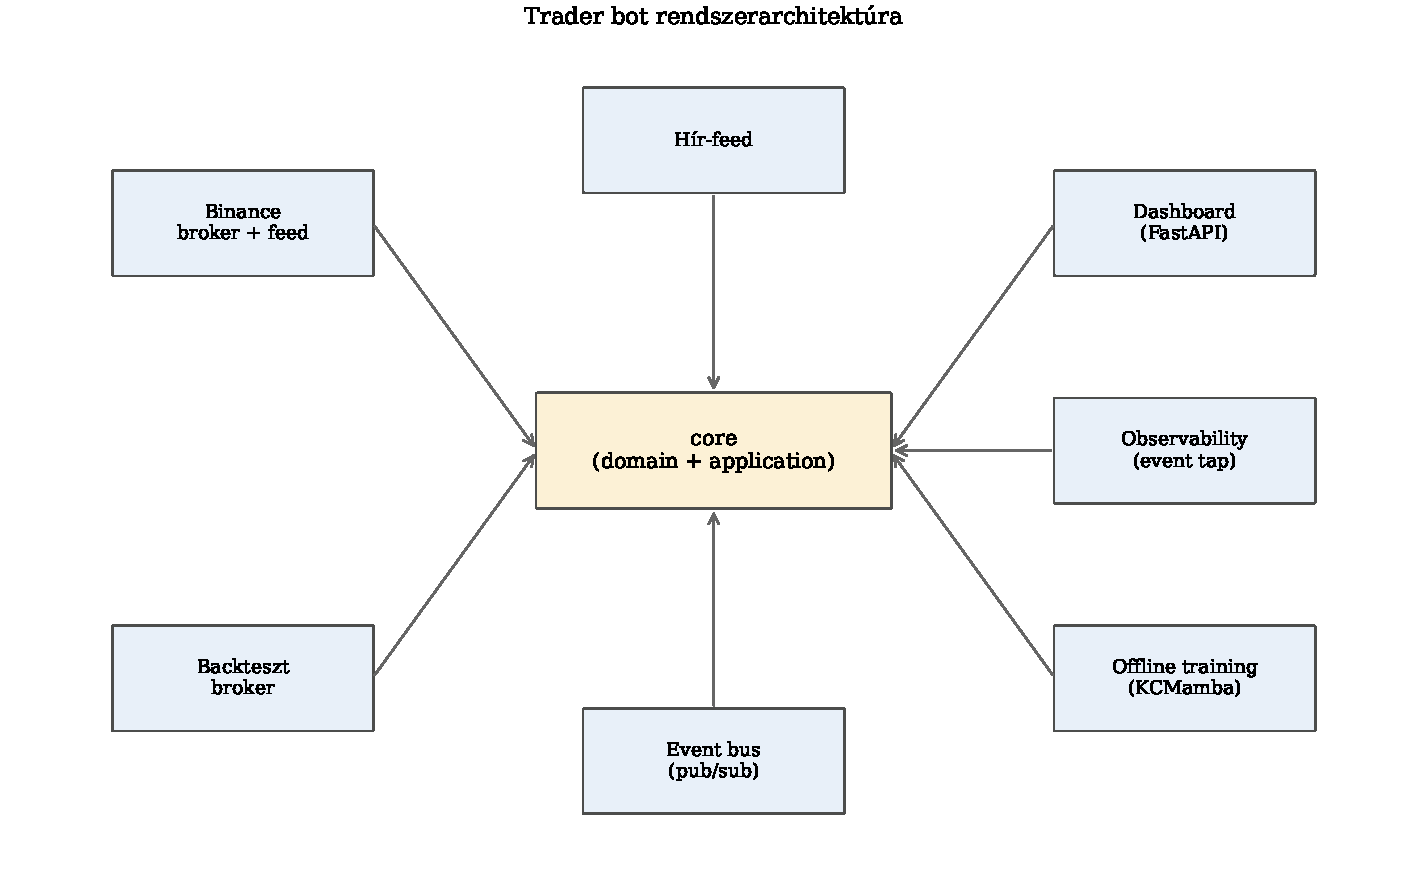
\includegraphics[width=\textwidth]{images/fig14_system_arch_hu.pdf}
  \caption{A KCMamba alapú kereskedési rendszer hexagonális architektúrájának
           áttekintése. A \textbf{Core} csomag tartalmazza a TradingEngine-t
           (pipeline: állapotbecslés $\to$ predikció $\to$ szignál $\to$ kockázat
           $\to$ végrehajtás), a domain modelleket és az alkalmazásportokat.
           A külső adapterek (Infrastructure, Web, Testing, Offline Training,
           Observability, Analytics) kizárólag az interfészeken ($\texttt{IEventBusPort}$,
           $\texttt{IBrokerGatewayPort}$ stb.) keresztül kommunikálnak a Core-ral.}
  \label{fig:system_arch}
\end{figure}

% ─────────────────────────────────────────────────────────────────────────────
\section{Modul- és osztályszerkezet}
\label{sec:module_structure}
% ─────────────────────────────────────────────────────────────────────────────

A forráskód négy fő csomagra oszlik. A \texttt{core/} nem hivatkozik
egyetlen adapterre sem. Az \texttt{adapters/} kód kizárólag a
\texttt{ports.py} interfészeken keresztül éri el.

\begin{table}[H]
  \centering
  \footnotesize
  \renewcommand{\arraystretch}{1.25}
  \begin{tabular}{|l|p{4.2cm}|p{6.3cm}|}
    \hline
    \textbf{Csomag} & \textbf{Modul / osztály} & \textbf{Felelősség} \\
    \hline\hline
    \multirow{4}{*}{\texttt{core/domain/}}
      & \texttt{models.py}      & Adattípusok: \texttt{Candle}, \texttt{Position}, \texttt{Order}, \texttt{Fill} \\
      & \texttt{strategy.py}    & \texttt{ThresholdStrategy}: Buy/Sell jelzéslogika,
                                  \texttt{min\_edge}, \texttt{max\_sigma} szűrők \\
      & \texttt{risk.py}        & \texttt{RiskPolicy}: kockázati szabálykészlet
                                  (MaxQty, Stop-loss, napi veszteség-limit) \\
      & \texttt{events.py}      & Domain-események: \texttt{PriceEvent},
                                  \texttt{SignalEvent}, \texttt{FillEvent} \\
    \hline
    \multirow{5}{*}{\texttt{core/application/}}
      & \texttt{engine.py}      & \texttt{TradingEngine}: fő pipeline-orkesztrálő,
                                  belső állapotgép a kereskedési ciklushoz \\
      & \texttt{execution.py}   & Megbízás-összeállítás, méretszámítás és
                                  \texttt{IBrokerGatewayPort}-ra küldés \\
      & \texttt{ports.py}       & Absztrakt interfészek:
                                  \texttt{IEventBusPort}, \texttt{IBrokerGatewayPort},
                                  \texttt{IMarketFeedPort}, \texttt{ITimeSourcePort} \\
      & \texttt{stages.py}      & Pipeline lépések: \texttt{PredictionStage},
                                  \texttt{SignalStage}, \texttt{RiskStage},
                                  \texttt{ExecutionStage} \\
      & \texttt{stores.py}      & In-memory állapot: \texttt{PositionStore},
                                  \texttt{SignalStore}, \texttt{EquityStore} \\
    \hline
    \multirow{4}{*}{\texttt{core/ml/}}
      & \texttt{kc\_mamba.py}         & \texttt{KCMambaModel}: PyTorch modul,
                                          \texttt{forward(x)} → előrejelzés \\
      & \texttt{mamba\_kalman.py}      & \texttt{KCMambaBlock}: Kalman-szűrő réteg,
                                          párhuzamos prefix-scan \\
      & \texttt{services.py}           & \texttt{MLService}: modellbetöltés,
                                          online frissítés, előrejelzés-gyorsítótár \\
      & \texttt{feature\_engineering.py} & OHLCV → jellemzővektor transzformáció,
                                            normalizáció, csúszóablak \\
    \hline
    \multirow{5}{*}{\texttt{adapters/}}
      & \texttt{binance\_broker.py}    & \texttt{BinanceBroker}: élő megbízás-végrehajtás
                                          REST API-n \\
      & \texttt{binance\_feed.py}      & \texttt{BinanceFeed}: WebSocket árfolyam-stream,
                                          reconnect logika \\
      & \texttt{event\_bus.py}         & \texttt{InMemoryEventBus}: aszinkron,
                                          \texttt{asyncio}-alapú eseménytovábbítás \\
      & \texttt{broker.py} (testing)   & \texttt{PaperBroker}, \texttt{SimulationWallet}:
                                          szimulált végrehajtás visszateszteléshez \\
      & \texttt{dashboard.py} (web)    & \texttt{DashboardServer}: aiohttp HTTP/WS
                                          szerver, REST JSON végpontok \\
    \hline
  \end{tabular}
  \caption{A rendszer modul- és osztályszerkezete. Minden osztály kizárólag a
           saját csomagjának adattípusaira és interfészeire támaszkodik.
           A keresztirányú függőségeket a \texttt{ports.py} absztrakciói
           közvetítik.}
  \label{tab:module_structure}
\end{table}

\cleardoublepage

% ============================================================
%  4. fejezet, Kísérletek és értékelés
% ============================================================
\chapter{Kísérletek és értékelés}
\label{ch:kiserletek}

\section{Kísérleti beállítások}
\label{sec:exp_setup}

\subsection{Hardver és szoftver}

A futtatási környezet: NVIDIA GeForce RTX 3060 (12~GB VRAM), PyTorch~2.x,
CUDA~12, float32 pontosság.

\subsection{Adatkészletek}
\label{sec:datasets}

A fő kérdezés három adatkészlet körnékeződött (részletes leírás a
\ref{sec:datasets}.~alfejezetben):

\begin{itemize}
    \item \textbf{Exchange-Rate}, 8 valutaárfolyam, 1990--2016
          (7\,588 nap, 8 változó)~\cite{lai2018modeling}.
    \item \textbf{ETTh1}, kínai transzformátorállomás, óránkénti terhelés
          és hőmérséklet (17\,420 lépés, 7 változó)~\cite{zhou2021informer}.
    \item \textbf{ETTh2}, ugyanaz az állomás, másik csatorna-sorozat
          (17\,420 lépés, 7 változó)~\cite{zhou2021informer}.
\end{itemize}

A \textbf{Weather} (21 meteorológiai változó, 52\,696 lépés) és az \textbf{ECL}
(321 csatorna, 26\,304 lépés) benchmarkok a nagyobb dimenzióság és a hosszú
periodicitás vizsgálatára következő mérési lépésben skálázandók; a jelen
dolgozat keretein belül csak a három fenti adatkészleten futó eredmények
szerepelnek, mert a tanulási futamok száma ($4$ zajszint $\times$ $2$ stride
$\times$ $4$ modell $\times$ $3$ adat = $96$ futam) már így is nagyobb, mint
amit egyetlen RTX 3060 hardverrel éssszerű időn belül elvégeztem.

\subsection{Zajmodell}

A zajosítás analítikusan:
\begin{equation}
    \hat{x} = x + \varepsilon,\qquad
    \varepsilon \sim \mathcal{N}(0, \sigma^2 I),\qquad
    \sigma \in \{0, 1, 3, 5\}.
\end{equation}
A tanító- és teszthalmazt azonos $\sigma$-val zajosítottam, így a vizsgált
probléma nem domain-shift, hanem egységes adatminőség-romlás.

\subsection{Modellkonfiguráció és tanítási hiperparaméterek}

\begin{table}[H]
    \centering
    \begin{tabular}{|l|c|c|c|}
        \hline
        \textbf{Hiperparaméter} & \textbf{LSTM} & \textbf{Fair Mamba} & \textbf{KCMamba} \\
        \hline\hline
        Epoch                & 5      & 5      & 5 \\
        Optimalizáló         & Adam   & Adam   & Adam \\
        Tanulási sebesség    & 3e-3   & 3e-3   & 3e-3 \\
        Kötegméret           & 32     & 32     & 32 \\
        Szekvenciahossz      & 96     & 96     & 96 \\
        Előrejelzési horizont & 96    & 96     & 96 \\
        Rejtett dim ($d$)    & 128    & 128    & 128 \\
        Fejek ($H$)          & n.a.      & 4      & 4 \\
        Állapotméret ($D$)   & n.a.      & 32     & 32 \\
        Rétegek              & 1      & 2      & 2 \\
        Kernel               & n.a.      & 4      & 4 \\
        \hline
        Paraméterek          & 71{,}0k & 53{,}2k & 46{,}1k \\
        \hline
    \end{tabular}
    \caption{Modell-konfigurációk és tanítási hiperparaméterek a zajrobusztussági
             kísérletekhez. A KCMamba kevesebb paraméterrel rendelkezik, mint a
             Fair Mamba, köszönhetően a kompaktabb Kalman-hálózatoknak.}
    \label{tab:hyperparams}
\end{table}

A stride ($s$) az ablak-eltolás lépése: $s=1$ esetén minden pozíció
tréningpéldává válik, $s=16$-nál nagyjából tizenhatszor kevesebb ablak keletkezik.

A fix $3\times 10^{-3}$ tanulási sebesség választását egy Smith-féle
\emph{learning rate range test}~\cite{smith2017cyclical} előzte meg: a
loss érzékeny tartománya mindhárom modellnél a $[10^{-3}, 10^{-2}]$
intervallumra esett, így ennek alsó felét választottam konzervatív
alapértéknek. Mivel a három modell loss-görbéje hasonló minőségű volt,
a továbbiakban azonos LR-rel tanítottam mindet a fér modellek
összehasonlíthatósága kedvéért.

\section{Eredmények}
\label{sec:results}

A bemutatást azzal a konfigurációval kezdem, ahol a KCMamba előnye a legnagyobb:
Exchange-Rate, $s=16$ stride mellett. Ez a beállítás két strukturlis tényezőt
kombinál: (i) a dataset kis méretű (7\,588 napi megfigyelés, mindegyik változónál
erős trend és gyenge periódus) és (ii) a $s=16$ stride további tizenhatszoros
ablakritkítást tesz, vagyis a zajmodell feltanításához eleve kevés példa áll
rendelkezésre. Így az az architektúrális döntés, hogy a zaj/jel szétválasztást
explicit $Q/R$ paraméterezéssel végezzük a Mamba szelektív gate-jei helyett,
komoly induktive többletet jelent.

\subsection{Exchange-Rate adatkészlet}

\begin{table}[H]
    \centering
    \small
    \begin{tabular}{|l|c|cccc|r|}
        \hline
        \textbf{Stride} & \textbf{Modell} &
        $\sigma=0$ & $\sigma=1$ & $\sigma=3$ & $\sigma=5$ & \textbf{Degr.} \\
        \hline\hline
        \multirow{4}{*}{$s=1$}
            & LSTM      & 0.219 & 0.664 & 0.922 & 1.139 & +421\% \\
            & Fair      & 0.022 & 0.381 & 0.979 & 1.757 & +7\,833\% \\
            & KCMamba       & 0.022 & 0.496 & \textbf{0.860} & \textbf{1.228} & +5\,505\% \\
            & ARIMA     & \textbf{0.004} & \textbf{0.176} & 1.716 & 5.430 & \cellcolor{red!20}+146\,461\% \\
        \hline
        \multirow{4}{*}{$s=16$}
            & LSTM      & 0.853 & 0.966 & 1.125 & 1.372 & +61\% \\
            & Fair      & 0.004 & 1.332 & 3.248 & 5.950 & \cellcolor{red!20}+152\,350\% \\
            & KCMamba       & 0.788 & \textbf{0.750} & \textbf{1.264} & \textbf{1.307} & \cellcolor{green!20}+66\% \\
            & ARIMA     & \textbf{0.003} & 0.782 & 6.721 & 20.774 & \cellcolor{red!20}+631\,340\% \\
        \hline
    \end{tabular}
    \caption{MSE értékek az Exchange adatkészleten különböző zajszinteken.
             Félkövérrel a legjobb (legkisebb MSE) érték zajszintenként.
             A ``Degr.'' oszlop a $\sigma=0 \to \sigma=5$ degradáció relatív mértéke.}
    \label{tab:exchange}
\end{table}

A $s=16$ konfiguráció mutatja a legmarkánsabb különbséget: az ARIMA
$\sigma=0$-nál a legjobb MSE-t éri el ($0.003$), ám $\sigma=5$ esetén
$+631\,340\%$-os degradációt ($6\,314\times$) szenved el. A neurális modellek
közül a Fair Mamba a legjobb zajmentes értéket adja ($\sigma=0$: MSE $= 0.004$),
de a $\sigma=5$ szinten az MSE-je $1\,487$-szeresére nő
($+152\,350\%$). A KCMamba degradációja $+66\%$, ami több nagyságrenddel
alacsonyabb érték.

A viselkedés a tanult $K$-gain dinamikájából következik: $\sigma=0$-nál
$K=0.706$, $\sigma=5$-nél $K=0.073$ ($A=0.926$). Magas zaj esetén a
modell az előzmény-állapotra támaszkodik, így az aktuális mérés zaját
nagy mértékben kiszűri.

\begin{table}[H]
    \centering
    \small
    \begin{tabular}{|l|c|cccc|r|}
        \hline
        \textbf{Stride} & \textbf{Modell} &
        $\sigma=0$ & $\sigma=1$ & $\sigma=3$ & $\sigma=5$ & \textbf{Degr.} \\
        \hline\hline
        \multirow{4}{*}{$s=1$}
            & LSTM      & \textbf{0.175} & \textbf{0.455} & \textbf{0.858} & \textbf{1.264} & +624\% \\
            & Fair      & 0.288 & 0.534 & 0.928 & 1.266 & \textbf{+339\%} \\
            & KCMamba       & 0.180 & 0.559 & 1.092 & 1.363 & +658\% \\
            & ARIMA     & 0.178 & 0.539 & 2.072 & 4.739 & +2\,566\% \\
        \hline
        \multirow{4}{*}{$s=16$}
            & LSTM      & 0.234 & \textbf{0.399} & \textbf{0.760} & \textbf{1.010} & +331\% \\
            & Fair      & \textbf{0.181} & 0.525 & 1.698 & 3.470 & +1\,817\% \\
            & KCMamba       & 0.189 & 0.453 & 0.856 & 1.120 & \textbf{+492\%} \\
            & ARIMA     & 0.191 & 0.623 & 6.010 & 18.638 & \cellcolor{red!20}+9\,653\% \\
        \hline
    \end{tabular}
    \caption{MSE értékek az ETTh1 adatkészleten. Az LSTM erős baseline-nak
             bizonyul nagy adatmennyiség és magas zaj esetén is.}
    \label{tab:etth1}
\end{table}

Az ETTh1 az LSTM erősebb adata: $s=1$-nél, ahol sok tréningpéldát lát,
mindkét zajszinten vezet. A KCMamba és a Fair Mamba alacsony zajnál hasonló
szinten van. $s=16$-nál a Fair Mamba $\sigma \ge 3$ esetén összeomlik
($+1\,817\%$), a KCMamba $+492\%$-on marad.

\subsection{ETTh2 adatkészlet}

\begin{table}[H]
    \centering
    \small
    \begin{tabular}{|l|c|cccc|r|}
        \hline
        \textbf{Stride} & \textbf{Modell} &
        $\sigma=0$ & $\sigma=1$ & $\sigma=3$ & $\sigma=5$ & \textbf{Degr.} \\
        \hline\hline
        \multirow{4}{*}{$s=1$}
            & LSTM      & 0.056 & 0.183 & 0.432 & 0.674 & +1\,098\% \\
            & Fair      & 0.079 & \textbf{0.174} & \textbf{0.476} & \textbf{0.808} & \textbf{+919\%} \\
            & KCMamba       & 0.056 & 0.206 & 0.512 & 0.871 & +1\,463\% \\
            & ARIMA     & \textbf{0.047} & 0.237 & 1.515 & 4.182 & \cellcolor{red!20}+8\,895\% \\
        \hline
        \multirow{4}{*}{$s=16$}
            & LSTM      & 0.146 & \textbf{0.225} & \textbf{0.392} & \textbf{0.545} & +274\% \\
            & Fair      & 0.050 & 0.351 & 1.238 & 3.108 & +6\,145\% \\
            & KCMamba       & 0.055 & 0.232 & 0.456 & 0.592 & \textbf{+982\%} \\
            & ARIMA     & \textbf{0.048} & 0.333 & 6.180 & 15.891 & \cellcolor{red!20}+33\,284\% \\
        \hline
    \end{tabular}
    \caption{MSE értékek az ETTh2 adatkészleten. Az ARIMA $\sigma=0$-nál mindkét
             stride esetén legjobb ($s=1$: 0.047, $s=16$: 0.048), de nagy zajnál
             összeömlik. A KCMamba nyeri a $s=16$ versenyt $\sigma=5$-nél (0.592 vs Fair 3.108).}
    \label{tab:etth2}
\end{table}

\subsection{Összefoglaló degradációs statisztika}

A három adatkészlet 24 konfigurációját aggregálva a $\sigma=0 \to \sigma=5$
átmenet relatív MSE-romlása adja a zajrobusztussági mérőszámot
(\ref{tab:degradation}.~táblázat).

\begin{table}[H]
    \centering
    \begin{tabular}{|l|r|r|r|}
        \hline
        \textbf{Modell} & \textbf{Átl.\ degradáció} & \textbf{Min} & \textbf{Max} \\
        \hline\hline
        LSTM             & $+468\%$             & $+61\%$      & $+1\,098\%$ \\
        \textbf{KCMamba} & $\mathbf{+1\,528\%}$ & $+66\%$      & $+5\,505\%$ \\
        Fair Mamba       & $+28\,234\%$         & $+339\%$     & $+152\,350\%$ \\
        ARIMA            & $+138\,700\%$        & $+2\,566\%$  & $+631\,340\%$ \\
        \hline
    \end{tabular}
    \caption{Átlagos MSE-degradáció $\sigma=0 \to \sigma=5$ zajszint-növelésnél.
             A KCMamba zajállósága $18{,}5\times$ jobb, mint a Fair Mambáé.}
    \label{tab:degradation}
\end{table}

\section{A Kalman-gain dinamikája}
\label{sec:k_dynamics}

A legmeggyőzőbb bizonyíték az Exchange/$s=16$ konfiguráció $K/A/R$ dinamikája
(\ref{tab:k_dynamics}.~táblázat):

\begin{table}[H]
    \centering
    \begin{tabular}{|c|c|c|c|}
        \hline
        $\sigma$ & $K_\text{avg}$ & $A = 1-K$ & $R_\text{avg}$ \\
        \hline\hline
        0{,}0 & 0{,}706 & 0{,}294 & 0{,}129 \\
        1{,}0 & 0{,}387 & 0{,}613 & 0{,}331 \\
        3{,}0 & 0{,}164 & 0{,}836 & 0{,}464 \\
        5{,}0 & 0{,}073 & 0{,}927 & 0{,}548 \\
        \hline
    \end{tabular}
    \caption{A KCMamba adaptív Kalman-gain értékei az Exchange/$s=16$
             konfigurációban. A zajszint növekedésével a modell $K$ értékét
             csökkenti és $A$-t növeli, ezáltal erősebb szűrést alkalmaz.}
    \label{tab:k_dynamics}
\end{table}

Amennyiben $R \gg Q$, a Kalman-szűrő az aktuális mérés helyett az
előzmény-állapotra támaszkodik. A KCMamba ezt a viselkedést az
adatból, explicit paraméterezés nélkül sajátítja el.

\section{Diszkusszió}

A Fair Mamba nagy zajnál azért omlik össze, mert a $K$-mechanizmus hiányában
a $\Delta, B, C$ paramétereknek egyidejűleg kell modellezniük az
adatstruktúrát és a zajt. Alacsony zajszinten ez a kettős feladat
működik, mert az adatból kiszűrhető elegendő hasznos jel. Magas zajnál
viszont a gradiens a $\Delta$ gate-et arra irányítja, hogy elhanyagolja
a bemenetet ($A \to 0$), ami zajmentes esetben katasztrofálisan rontja
az előrejelzést: a modell elveszti a bemeneti jel követésének képességét,
és kvázi konstans kimenetet produkál.

A KCMamba előnye ritka adat mellett lesz valóban szembetűnő. Az Exchange/$s=16$
konfiguráció egyszerre ötvözi a kis adatkészletet (7\,588 nap) és a nagy
stride-ból adódó tizenhatszoros ablakritkítást, így a tanítás során rendkívül
kevés példa áll rendelkezésre a zajszerkezet implicit megtanulásához.
Az explicit $Q/R$ dekompozíció ilyen körülmények között erős priorként
viselkedik: a modellnek nem kell a zajmodellt tisztán az adatból
előállítania, mert az architekturális szinten be van építve. Ez magyarázza
a $+66\%$ vs Fair $+152\,350\%$ különbséget ugyanazon a futásokon.

Az LSTM sok adaton és magas zajszinten egyaránt jól teljesít, mert a
forget/input gate együttese tanult súlyokkal (explicit Kalman-struktúra
nélkül) hasonló adaptív szűrési hatást valósít meg. A 96 lépéses
előrejelzési horizonton az LSTM memória-korlátai még nem dominánsak;
ezek hatása hosszabb szekvenciáknál várható.

\cleardoublepage

% ============================================================
%  5. fejezet, Összegzés
% ============================================================
\chapter{Összegzés}
\label{ch:osszegzes}

\section{Főbb eredmények}

A KCMamba architektúra differenciálható Kalman-szűrési mechanizmust
integrál a Mamba SSM-be. A három adatkészleten végzett kísérletekből
az alábbi következtetések vonhatók le:

\begin{enumerate}
    \item Zajrobusztusság: $\sigma=0 \to \sigma=5$ zajszint-növelésnél
          a KCMamba átlagos MSE-degrádációja $+1\,528\%$, a Fair Mambáé $+28\,234\%$,
          ami $18{,}5\times$-os különbség. Exchange/$s=16$-nál
          a különbség öt nagyságrend: $+66\%$ vs $+152\,350\%$.

    \item Kalman-gain adaptáció: a modell által az adatokból
          megtanult $K$-érték a zajszint emelkedésével monoton csökken
          ($0.706 \to 0.073$), ami konzisztens az explicit Kalman-egyenletekből
          származtatható várakozásokkal. Ez megerősíti, hogy az architekturális
          prior érdemben irányítja a tanulási folyamatot.

    \item Kevés adat: $s=16$ stride esetén a Kalman-struktúra
          implicit regularizáló hatást fejt ki, ami ellensúlyozza
          az adathiányt.
\end{enumerate}

\section{Korlátok}

A KCMamba nem minden konfigurációban jobb, és a kísérleti keretrendszer
több olyan egyszerűsítést tartalmaz, amelyek a következtetések
általánosíthatóságát érdemben korlátozzák.

\begin{itemize}
    \item Zajtalan, kis stride esetén ($\sigma=0$, $s=16$) a Fair Mamba
          szinte memorizál, és itt az MSE-je sokkal jobb. Ez arra utal,
          hogy az explicit Kalman-struktúra zajtalan környezetben
          felesleges overheadet jelent: a mindig jelen lévő szűrési tag
          enyhe alulilleszkedést okoz, és a struktúra nem képes teljesen
          kikapcsolni a szűrést.

    \item ETTh1/$s=1$-nél az LSTM a legjobb; a gating mechanizmus
          kihasználja a nagy adatmennyiséget. Az LSTM forget/input gate
          párosa hasonló adaptív szűrést valósít meg, de rugalmasabb, mert
          nem köti meg a $K = Q/(Q+R)$ struktúra. Ez nem a KCMamba
          kudarca, hanem annak illusztrációja, hogy adatgazdag rezsimben
          az induktív prior haszna csökken.

    \item Mindössze 5 epoch futott, és minden konfigurációt csak egyetlen
          magon (seed) futtattam. Ez sem a konvergált állapotot, sem a
          statisztikai szignifikanciát nem garantálja: a bemutatott
          eredmények pontbecslések, konfidencia-intervallum nélkül.
          Publikációérett tanulmány legalább három ismétlést és korai
          leállítást igényelne.

    \item Csak $L=H=96$ horizontot vizsgáltam. A 336, 720 és 960 lépéses
          horizontokon a Mamba $O(T)$ komplexitása számottevő előnyt hozhat
          az $O(T^2)$ Transzformerekkel szemben, és az LSTM memória-korlátai
          is itt kezdenek dominálni; a jelen fejezet következtetései
          tehát formálisan csak a rövid horizontra vonatkoznak.

    \item A zajmodell kizárólag izotróp Gauss-zaj
          ($\varepsilon \sim \mathcal{N}(0, \sigma^2 I)$); a valós alkalmazásokban
          a zaj jellemzően heteroszkedasztikus, időben korrelált, esetenként
          nem-Gauss eloszlású, és gyakran strukturális (szenzorkiesés, hiányzó
          érték). Az itt mért robusztusság ezekre a zajformákra nem
          általánosítható automatikusan.

    \item A skalár $Q_t$, $R_t$ becslés feltételezi, hogy a zajkomponensek
          csatornánként függetlenek. Diagonális vagy teljes kovarianciamátrix
          becslése gazdagabb zajmodellt eredményezne, de a paraméterszámot
          érzékelhetően növelné.

    \item Két benchmark (Weather, ECL) a tanítási futamszám skálázódása
          miatt a jelen kísérleti körbe nem került be; a dimenzió-érzékenység
          (7 vs.\ 21 vs.\ 321 csatorna) \emph{a~priori} nincs alátámasztva.

    \item A hiperparaméter-érzékenység szélesebb körű vizsgálata (rejtett
          dimenzió, fejek száma, rétegek száma, kernelméret, tanulási sebesség)
          nem történt meg; a bemutatott konfiguráció egy ésszerű alapbeállítás,
          amely nem biztos, hogy Pareto-optimális.

    \item A valós kereskedelmi oldalon (\ref{ch:implementacio}.\ fejezet)
          a rendszer backtestben van validálva; élő piac, slippage-ingadozás,
          szünetek és részteljesülési sorrend-hatások a jelen dolgozat
          hatókörén kívül esnek.
\end{itemize}

\section{Jövőbeli irányok}

\begin{itemize}
    \item Az $s \in \{1, 4, 8, 16, 32, 64\}$ értékek szisztematikus
          végigpásztázása megmutatná, melyik adatszegénységi küszöbnél
          jelenik meg először a Kalman-struktúra szabályozó hatása.

    \item 336, 720, illetve 960 lépéses előrejelzési horizonton
          a Mamba $O(T \log T)$ komplexitása számottevő előnyt hozhat
          az $O(T^2)$ Transzformerekkel szemben.

    \item A szimulált Gauss-zaj szenzorkiesésekkel, hiányzó értékekkel
          és kilógó megfigyelésekkel való felváltása az architektúrát
          a valós alkalmazási feltételekhez közelítené.

    \item Egy meta-hálózat alapú zajszint-becslés lehetővé tenné,
          hogy $\sigma$ tanított paraméterré váljon, és a modell
          ismeretlen zajú környezetekhez automatikusan alkalmazkodjon.

    \item A skalár $Q_t$, $R_t$ diagonális Cholesky-faktorizációval
          való felváltása gazdagabb bizonytalanság-becslést és
          jobb kalibrációt eredményezhet.
\end{itemize}

\section{Zárszó}

A KCMamba eredményei arra mutatnak rá, hogy a klasszikus Kalman-szűrési
elvek és a modern szekvencia-modellek nem egymást kizáró megközelítések,
hanem produktívan összekapcsolhatók.
Az explicit zajmodell olyan induktív torzítást visz az architektúrába,
amely előnyt jelent a korlátozott adatmennyiségű és/vagy magas
zajszintű körülmények között.
A~\ref{ch:implementacio}. fejezetben ismertetett rendszer azt is
igazolja, hogy a modell valós kereskedési környezetbe integrálható,
nem csak kísérleti körülmények között használható.

\cleardoublepage

% Köszönetnyilvánítás
\chapter*{\acklabel}
\addcontentsline{toc}{chapter}{\acklabel}
A szerző köszönetét fejezi ki a témavezetőnek a szakmai iránymutatásért,
valamint az ELTE Informatikai Karának a kutatási infrastruktúra biztosításáért.
Külön köszönet illeti az idősor-előrejelzési közösséget a nyílt adatkészletekért
(ETTh1, ETTh2, Exchange-Rate), amelyek nélkül az empirikus értékelés nem lett volna lehetséges.

% ─── SAJÁT EREDMÉNYEK NYILATKOZATA (OTDK kötelező) ───────────────────────────
\chapter*{A saját eredmények lehatárolása}
\addcontentsline{toc}{chapter}{A saját eredmények lehatárolása}

Az alábbi táblázat az OTDK~37 előírásainak megfelelően egyértelműen elkülöníti
a pályázó hallgató saját eredményeit a témavezető, illetve a tágabb kutatócsoport
eredményeitől.

\begin{center}
\begin{tabular}{|p{7.0cm}|p{7.0cm}|}
\hline
\textbf{Kovács András saját eredményei} & \textbf{Témavezető / irodalom} \\
\hline
A KCMamba architektúra teljes tervezése: a
$Q_\text{net}$-, $R_\text{net}$-, $K_\text{net}$-alhálózatok,
az adaptív Kalman-gate mechanizmus és a
heteroszkedasztikus NLL-veszteségfüggvény kidolgozása. &
A Mamba és S4 alaparchitektúra publikált eredményei
\cite{gu2023mamba,gu2021s4}. \\
\hline
A Fair~Mamba baseline megtervezése és implementálása,
amely azonos paraméterszámon biztosít igazságos összehasonlítást. &
Az LTSF-Linear, iTransformer és egyéb baseline-ok
az irodalomból \cite{zeng2023transformers,liu2023itransformer}. \\
\hline
A kísérleti protokoll kialakítása: 9~zajtípus,
kiterjesztett $T/s$ rács, ablációs vizsgálat,
Wilcoxon-szignifikancia-tesztek. &
A nyílt adatkészletek (ETTh1/h2/m1, Exchange-Rate,
Weather stb.) és a sztenderd MSE/MAE metrikák. \\
\hline
A teljes szoftverrendszer önálló fejlesztése:
aszinkron kereskedési motor, visszatesztelő
keret, Binance-adapter, webes irányítópult. &
Témavezetői konzultációk és szakmai visszajelzések
a fejlesztési folyamat során. \\
\hline
\end{tabular}
\end{center}

% ============================================================
%  FÜGGELÉKEK
% ============================================================
\appendix
% A_hyperparams és B_teljes_tablazatok elhagyva
% % ============================================================
%  Függelék A, Hiperparaméter táblázatok
% ============================================================
\chapter{Hiperparaméterek}
\label{app:hyperparams}

Ez a függelék az összes kísérletben alkalmazott hiperparaméter teljes listáját
tartalmazza.

\section{Közös tanítási beállítások}

\begin{table}[H]
    \centering
    \begin{tabular}{|l|l|l|}
        \hline
        \textbf{Paraméter} & \textbf{Érték} & \textbf{Megjegyzés} \\
        \hline\hline
        Epoch                  & 5          & Gyors teszt, produkció: 20–50 \\
        Optimalizáló           & Adam       & $\beta_1=0.9$, $\beta_2=0.999$ \\
        Tanulási sebesség      & $3 \times 10^{-3}$ & Nincs scheduler \\
        Kötegméret             & 32         & \\
        Szekvenciahossz        & 96         & lookback ablak \\
        Előrejelzési horizont  & 96         & \\
        Loss függvény          & MSELoss    & PyTorch, reduction=mean \\
        Eszköz                 & CUDA (GPU) & RTX 3060 12 GB \\
        Adattípus              & float32    & \\
        \hline
    \end{tabular}
    \caption{Közös tanítási hiperparaméterek az összes modellhez.}
    \label{tab:app_train}
\end{table}

\section{LSTM hiperparaméterek}

\begin{table}[H]
    \centering
    \begin{tabular}{|l|l|}
        \hline
        \textbf{Paraméter} & \textbf{Érték} \\
        \hline\hline
        Rejtett méret (\texttt{hidden\_size}) & 128 \\
        Rétegek száma (\texttt{num\_layers})  & 1 \\
        Dropout                               & 0 \\
        Kétirányú (\texttt{bidirectional})    & Nem \\
        Projekciós réteg (head)               & Linear($128 \to$ pred\_len $\times$ channels) \\
        Paraméterek száma                     & 71\,730 \\
        \hline
    \end{tabular}
    \caption{LSTM modell hiperparaméterek.}
    \label{tab:app_lstm}
\end{table}

\section{Fair Mamba hiperparaméterek}

\begin{table}[H]
    \centering
    \begin{tabular}{|l|l|}
        \hline
        \textbf{Paraméter} & \textbf{Érték} \\
        \hline\hline
        Modell dimenzió (\texttt{d\_model})    & 128 \\
        Fejek (\texttt{heads}, $H$)            & 4 \\
        Állapotméret (\texttt{d\_state}, $D$)  & 32 \\
        Belső dimenzió ($E = H \times D$)      & 128 \\
        Konvolúciós kernel (\texttt{d\_conv})  & 4 \\
        Rétegek száma                          & 2 \\
        dt inicializáció                       & \texttt{dt\_min}$=0.001$, \texttt{dt\_max}$=0.1$ \\
        Paraméterek száma                      & 53\,248 \\
        \hline
    \end{tabular}
    \caption{Fair Mamba modell hiperparaméterek.}
    \label{tab:app_fair}
\end{table}

\section{KCMamba hiperparaméterek}

\begin{table}[H]
    \centering
    \begin{tabular}{|l|l|}
        \hline
        \textbf{Paraméter} & \textbf{Érték} \\
        \hline\hline
        Modell dimenzió (\texttt{d\_model})    & 128 \\
        Fejek (\texttt{heads}, $H$)            & 4 \\
        Állapotméret (\texttt{d\_state}, $D$)  & 32 \\
        Belső dim ($E = H \times D$)           & 128 \\
        Konvolúciós kernel (\texttt{kernel\_size}) & 4 \\
        Rétegek száma                          & 2 \\
        $Q$ skálázó (\texttt{q\_scale})        & $-2.0$ \\
        $R$ skálázó (\texttt{r\_scale})        & $+1.5$ \\
        $K_\Delta$ amplitúdó                   & $0.3$ \\
        Reziduál kapu (\texttt{b\_res})        & $-1.0$ \\
        $K_\text{net}$ rejtett dim             & 64 \\
        Lassú stride (\texttt{slow\_stride})   & 4 \\
        Paraméterek száma                      & 46\,134 \\
        \hline
    \end{tabular}
    \caption{KCMamba modell hiperparaméterek. A $q\_\text{scale}$ és
             $r\_\text{scale}$ inicializáció $K_\text{base} \approx 0.07$-et
             eredményez, ami erős alapértelmezett szűrést biztosít.}
    \label{tab:app_kcmamba}
\end{table}

\section{Adat-előkészítési paraméterek}

\begin{table}[H]
    \centering
    \begin{tabular}{|l|l|l|}
        \hline
        \textbf{Paraméter} & \textbf{Érték} & \textbf{Megjegyzés} \\
        \hline\hline
        Normálás                  & StandardScaler   & Jellemzőnkénti z-score \\
        Train / val / test arány  & 70\% / 10\% / 20\% & Cronológiai split \\
        Stride ($s=1$)            & 1               & Maximális fedettség \\
        Stride ($s=16$)           & 16              & Ritka mintavétel \\
        Zaj-modell                & $\mathcal{N}(0, \sigma^2)$ & Additív \\
        Zaj alkalmazása           & Jellemzőkre      & Train + eval \\
        \hline
    \end{tabular}
    \caption{Adat-előkészítési paraméterek a zajrobusztussági kísérletekhez.}
    \label{tab:app_data}
\end{table}

% \cleardoublepage
% % ============================================================
%  Függelék B, Teljes eredménytáblázatok
% ============================================================
\chapter{Teljes kísérleti eredmények}
\label{app:full_results}

Ez a függelék az összes 24 konfiguráció részletes MSE eredményeit tartalmazza,
beleértve a tanítási időt és a KC-specifikus $K/A/R$ értékeket.

\section{Exchange adatkészlet, stride=1}

\begin{table}[H]
    \centering
    \small
    \begin{tabular}{|c|l|r|r|r|}
        \hline
        \textbf{Zaj ($\sigma$)} & \textbf{Modell} & \textbf{MSE} & \textbf{Idő (s)} & \textbf{K / A / R} \\
        \hline\hline
        \multirow{3}{*}{0.0}
            & LSTM      & 0.218776 & 1.8 & n.a. \\
            & Fair      & 0.022154 & 6.1 & n.a. \\
            & KCMamba & 0.021916 & 8.5 & 0.999 / 0.010 / 0.009 \\
        \hline
        \multirow{3}{*}{1.0}
            & LSTM      & 0.664242 & 1.9 & n.a. \\
            & Fair      & 0.381262 & 5.8 & n.a. \\
            & KCMamba & 0.496262 & 7.2 & 0.175 / 0.824 / 0.021 \\
        \hline
        \multirow{3}{*}{3.0}
            & LSTM      & 0.921943 & 1.4 & n.a. \\
            & Fair      & 0.978586 & 5.9 & n.a. \\
            & KCMamba & 0.859947 & 8.3 & 0.094 / 0.902 / 0.071 \\
        \hline
        \multirow{3}{*}{5.0}
            & LSTM      & 1.138875 & 1.9 & n.a. \\
            & Fair      & 1.757482 & 5.9 & n.a. \\
            & KCMamba & 1.228382 & 8.3 & 0.098 / 0.899 / 0.101 \\
        \hline
    \end{tabular}
    \caption{Exchange adatkészlet, stride=1: teljes MSE eredmények.}
    \label{tab:full_exchange_s1}
\end{table}

\section{Exchange adatkészlet, stride=16}

\begin{table}[H]
    \centering
    \small
    \begin{tabular}{|c|l|r|r|r|}
        \hline
        \textbf{Zaj ($\sigma$)} & \textbf{Modell} & \textbf{MSE} & \textbf{Idő (s)} & \textbf{K / A / R} \\
        \hline\hline
        \multirow{3}{*}{0.0}
            & LSTM      & 0.852632 & 0.1 & n.a. \\
            & Fair      & 0.003903 & 0.4 & n.a. \\
            & KCMamba & 0.787992 & 0.5 & 0.706 / 0.294 / 0.129 \\
        \hline
        \multirow{3}{*}{1.0}
            & LSTM      & 0.966091 & 0.1 & n.a. \\
            & Fair      & 1.331967 & 0.4 & n.a. \\
            & KCMamba & 0.750111 & 0.5 & 0.387 / 0.613 / 0.331 \\
        \hline
        \multirow{3}{*}{3.0}
            & LSTM      & 1.124837 & 0.1 & n.a. \\
            & Fair      & 3.248106 & 0.4 & n.a. \\
            & KCMamba & 1.264269 & 0.5 & 0.164 / 0.836 / 0.464 \\
        \hline
        \multirow{3}{*}{5.0}
            & LSTM      & 1.372140 & 0.1 & n.a. \\
            & Fair      & 5.950133 & 0.4 & n.a. \\
            & KCMamba & 1.306888 & 0.5 & 0.073 / 0.926 / 0.548 \\
        \hline
    \end{tabular}
    \caption{Exchange adatkészlet, stride=16: teljes MSE eredmények.
             A Fair Mamba $\sigma=5$-nél $5.950$ MSE-t ér el (+152\,350\% degradáció).}
    \label{tab:full_exchange_s16}
\end{table}

\section{ETTh1 adatkészlet, stride=1}

\begin{table}[H]
    \centering
    \small
    \begin{tabular}{|c|l|r|r|r|}
        \hline
        \textbf{Zaj ($\sigma$)} & \textbf{Modell} & \textbf{MSE} & \textbf{Idő (s)} & \textbf{K / A / R} \\
        \hline\hline
        \multirow{3}{*}{0.0}
            & LSTM      & 0.174678 & 3.5 & n.a. \\
            & Fair      & 0.288250 & 13.8 & n.a. \\
            & KCMamba & 0.179808 & 19.4 & 0.671 / 0.332 / 0.106 \\
        \hline
        \multirow{3}{*}{1.0}
            & LSTM      & 0.454999 & 3.5 & n.a. \\
            & Fair      & 0.533635 & 13.9 & n.a. \\
            & KCMamba & 0.558625 & 19.4 & 0.311 / 0.688 / 0.140 \\
        \hline
        \multirow{3}{*}{3.0}
            & LSTM      & 0.858074 & 3.4 & n.a. \\
            & Fair      & 0.928225 & 13.7 & n.a. \\
            & KCMamba & 1.092434 & 19.4 & 0.108 / 0.888 / 0.168 \\
        \hline
        \multirow{3}{*}{5.0}
            & LSTM      & 1.263812 & 3.5 & n.a. \\
            & Fair      & 1.265982 & 14.1 & n.a. \\
            & KCMamba & 1.363318 & 19.3 & 0.087 / 0.908 / 0.182 \\
        \hline
    \end{tabular}
    \caption{ETTh1 adatkészlet, stride=1: teljes MSE eredmények.}
    \label{tab:full_etth1_s1}
\end{table}

\section{ETTh1 adatkészlet, stride=16}

\begin{table}[H]
    \centering
    \small
    \begin{tabular}{|c|l|r|r|r|}
        \hline
        \textbf{Zaj ($\sigma$)} & \textbf{Modell} & \textbf{MSE} & \textbf{Idő (s)} & \textbf{K / A / R} \\
        \hline\hline
        \multirow{3}{*}{0.0}
            & LSTM      & 0.234299 & 0.2 & n.a. \\
            & Fair      & 0.181018 & 0.7 & n.a. \\
            & KCMamba & 0.189180 & 1.1 & 0.918 / 0.084 / 0.134 \\
        \hline
        \multirow{3}{*}{1.0}
            & LSTM      & 0.399315 & 0.2 & n.a. \\
            & Fair      & 0.524590 & 0.8 & n.a. \\
            & KCMamba & 0.452819 & 1.1 & 0.489 / 0.511 / 0.334 \\
        \hline
        \multirow{3}{*}{3.0}
            & LSTM      & 0.760479 & 0.2 & n.a. \\
            & Fair      & 1.697535 & 0.8 & n.a. \\
            & KCMamba & 0.856120 & 1.1 & 0.118 / 0.881 / 0.617 \\
        \hline
        \multirow{3}{*}{5.0}
            & LSTM      & 1.009729 & 0.2 & n.a. \\
            & Fair      & 3.469893 & 0.8 & n.a. \\
            & KCMamba & 1.119790 & 1.1 & 0.066 / 0.934 / 0.749 \\
        \hline
    \end{tabular}
    \caption{ETTh1 adatkészlet, stride=16: teljes MSE eredmények.}
    \label{tab:full_etth1_s16}
\end{table}

\section{ETTh2 adatkészlet, stride=1}

\begin{table}[H]
    \centering
    \small
    \begin{tabular}{|c|l|r|r|r|}
        \hline
        \textbf{Zaj ($\sigma$)} & \textbf{Modell} & \textbf{MSE} & \textbf{Idő (s)} & \textbf{K / A / R} \\
        \hline\hline
        \multirow{3}{*}{0.0}
            & LSTM      & 0.056229 & 3.0 & n.a. \\
            & Fair      & 0.079275 & 9.0 & n.a. \\
            & KCMamba & 0.055749 & 18.4 & 0.999 / 0.010 / 0.040 \\
        \hline
        \multirow{3}{*}{1.0}
            & LSTM      & 0.182996 & 3.5 & n.a. \\
            & Fair      & 0.174298 & 13.8 & n.a. \\
            & KCMamba & 0.205602 & 19.3 & 0.225 / 0.772 / 0.066 \\
        \hline
        \multirow{3}{*}{3.0}
            & LSTM      & 0.431764 & 3.5 & n.a. \\
            & Fair      & 0.475908 & 13.7 & n.a. \\
            & KCMamba & 0.512048 & 19.1 & 0.077 / 0.918 / 0.106 \\
        \hline
        \multirow{3}{*}{5.0}
            & LSTM      & 0.673502 & 3.5 & n.a. \\
            & Fair      & 0.807593 & 13.8 & n.a. \\
            & KCMamba & 0.871165 & 13.8 & 0.054 / 0.940 / 0.137 \\
        \hline
    \end{tabular}
    \caption{ETTh2 adatkészlet, stride=1: teljes MSE eredmények.}
    \label{tab:full_etth2_s1}
\end{table}

\section{ETTh2 adatkészlet, stride=16}

\begin{table}[H]
    \centering
    \small
    \begin{tabular}{|c|l|r|r|r|}
        \hline
        \textbf{Zaj ($\sigma$)} & \textbf{Modell} & \textbf{MSE} & \textbf{Idő (s)} & \textbf{K / A / R} \\
        \hline\hline
        \multirow{3}{*}{0.0}
            & LSTM      & 0.145848 & 0.2 & n.a. \\
            & Fair      & 0.049769 & 0.8 & n.a. \\
            & KCMamba & 0.054675 & 1.2 & 0.998 / 0.010 / 0.046 \\
        \hline
        \multirow{3}{*}{1.0}
            & LSTM      & 0.225112 & 0.2 & n.a. \\
            & Fair      & 0.350659 & 0.8 & n.a. \\
            & KCMamba & 0.231545 & 1.2 & 0.415 / 0.585 / 0.185 \\
        \hline
        \multirow{3}{*}{3.0}
            & LSTM      & 0.391637 & 0.2 & n.a. \\
            & Fair      & 1.237534 & 0.8 & n.a. \\
            & KCMamba & 0.456027 & 1.1 & 0.078 / 0.922 / 0.414 \\
        \hline
        \multirow{3}{*}{5.0}
            & LSTM      & 0.545204 & 0.2 & n.a. \\
            & Fair      & 3.108295 & 0.8 & n.a. \\
            & KCMamba & 0.591713 & 1.2 & 0.059 / 0.939 / 0.540 \\
        \hline
    \end{tabular}
    \caption{ETTh2 adatkészlet, stride=16: teljes MSE eredmények.}
    \label{tab:full_etth2_s16}
\end{table}

\section{Degradációs összefoglaló (mind a 6 konfiguráció)}

\begin{table}[H]
    \centering
    \begin{tabular}{|l|l|r|r|r|}
        \hline
        \textbf{Dataset} & \textbf{Stride} & \textbf{LSTM Degr.} & \textbf{Fair Degr.} & \textbf{KC Degr.} \\
        \hline\hline
        Exchange & $s=1$  & +421\%  & +7\,833\%   & +5\,505\% \\
        Exchange & $s=16$ & +61\%   & +152\,350\% & +66\% \\
        ETTh1    & $s=1$  & +624\%  & +339\%      & +658\% \\
        ETTh1    & $s=16$ & +331\%  & +1\,817\%   & +492\% \\
        ETTh2    & $s=1$  & +1\,098\% & +919\%    & +1\,463\% \\
        ETTh2    & $s=16$ & +274\%  & +6\,145\%   & +982\% \\
        \hline
        \textbf{Átlag}   &        & +468\%  & +28\,234\%  & +1\,528\% \\
        \hline
    \end{tabular}
    \caption{MSE degradáció $\sigma=0 \to \sigma=5$ esetén az összes konfigurációban.
             A KCMamba átlagos degradációja 18.5$\times$ kisebb, mint a Fair Mamba-é.
             A futási idő összesen: 6.3 perc (CUDA, 5 epoch/konfiguráció).}
    \label{tab:full_degradation}
\end{table}

% \cleardoublepage

% ─── AI-ESZKÖZÖK DOKUMENTÁCIÓJA (OTDK kötelező) ──────────────────────────────
\chapter{Mesterséges intelligencia alapú eszközök felhasználása}
\label{app:ai}

Az OTDK~37 felhívásának megfelelően az alábbiakban dokumentáljuk a pályamunka
készítése során igénybe vett mesterséges intelligencia alapú eszközöket és
azok felhasználási módját.

\begin{center}
\begin{tabular}{|p{3.5cm}|p{5.5cm}|p{4.5cm}|}
\hline
\textbf{Eszköz} & \textbf{Felhasználási mód} & \textbf{Érintett területek} \\
\hline
GitHub Copilot\newline(GPT-4o alapú) &
Kódkiegészítés és kódrészlet-generálás a Python implementáció során
(benchmark szkriptek, sweep logika, tesztek). &
Implementáció, kísérleti sweep \\
\hline
ChatGPT\newline(GPT-4o) &
Nyelvhelyesség-ellenőrzés, \LaTeX{} szintaxis-kérdések.
Tartalomgenerálásra \emph{nem} alkalmaztuk. &
Szövegszerkesztési segítség \\
\hline
\end{tabular}
\end{center}

\bigskip
\noindent
\textbf{Fontos megjegyzés:} Az eszközök kizárólag segédeszközként kerültek
alkalmazásra. A tudományos tartalom, az architektúra-tervezési döntések, a
kísérleti protokoll és az eredmények értelmezése teljes egészében a szerző
saját szellemi terméke. Az AI-eszközök által javasolt kódrészleteket minden
esetben a szerző ellenőrizte, tesztelte és szükség szerint módosította.

% Irodalomjegyzék (kötelező)
\phantomsection
\addcontentsline{toc}{chapter}{\biblabel}
\printbibliography[title=\biblabel]
\cleardoublepage

% Ábrajegyzék
\phantomsection
\addcontentsline{toc}{chapter}{Ábrajegyzék}
\listoffigures
\cleardoublepage

% ============================================================
\end{document}
